\documentclass[10pt]{article}
\usepackage[verbose, a4paper, hmargin=2.5cm, vmargin=2.5cm]{geometry}

\usepackage{fontspec}
\usepackage{ctex}
\usepackage{paratype}

\usepackage{amsmath}
\usepackage{amssymb}
\usepackage{amsfonts}
\usepackage{esint}
\usepackage{stmaryrd}

\usepackage[mathbf=sym]{unicode-math}
\usepackage{newunicodechar}
\setmainfont{STIX Two Text}
\setmathfont{STIX Two Math}
\newunicodechar{≤}{\ensuremath{\leq}}
\newunicodechar{≥}{\ensuremath{\geq}}
\newunicodechar{∈}{\ensuremath{\in}}
\newunicodechar{⊂}{\ensuremath{\subset}}

\setsansfont{Arial}
\setmonofont{Courier New}

\usepackage{makecell}
\usepackage{wasysym}
\usepackage{pifont}
\usepackage[export]{adjustbox}
\usepackage{graphicx}
\usepackage{mdframed}
\usepackage{booktabs,array,multirow}
\usepackage{tabularx}
\usepackage{hyperref}
\hypersetup{colorlinks=true, linkcolor=blue, filecolor=magenta, urlcolor=cyan,}
\urlstyle{same}
\usepackage[most]{tcolorbox}
\definecolor{mygray}{RGB}{240,240,240}
\tcbset{
  colback=mygray,
  boxrule=0pt,
}
\graphicspath{ {./images/} }
\newcommand{\HRule}{\begin{center}\rule{0.9\linewidth}{0.2mm}\end{center}}
\newcommand{\customfootnote}[1]{
  \let\thefootnote\relax\footnotetext{#1}
}
\newcommand{\lt}{\mathrel{<}}
\newcommand{\gt}{\mathrel{>}}
\newcommand*\circled[1]{\tikz[baseline=(char.base)]{\node[shape=circle,draw,inner sep=1.5pt] (char) {\small #1};}}
\setcounter{MaxMatrixCols}{256}
\begin{document}
Math-Net.Ru
Общероссийский математический портал

Л. С. Понтрягин, Математическая теория оптимальных
процессов и дифференциальные игры,
Тр. МИАН СССР, 1985, том 169, 119--158
https://www.mathnet.ru/tm2215
Использование Общероссийского математического портала Math-Net.Ru подразумевает, что вы прочитали и согласны с пользовательским соглашением
https://www.mathnet.ru/rus/agreement
Параметры загрузки:
IP: 109.252.165.210
20 декабря 2025 г., 04:14:31

Труды

Математического

1985,

том 169

УДК

517.978

института АН

СССР

Л . С.

ПОНТРЯГИН

МАТЕМАТИЧЕСКАЯ ТЕОРИЯ ОПТИМАЛЬНЫХ ПРОЦЕССОВ
И ДИФФЕРЕНЦИАЛЬНЫЕ ИГРЫ
В 1950 и 1951 гг. дирекция Математического института им. В. А. Стеклова
в лице зам. директора М. В. Келдыша и партийная организация института ста­
ли настойчиво рекомендовать мне заняться прикладными вопросами. Эта
рекомендация полностью соответствовала моим собственным взглядам. В 1932
и 1942 гг. я уже делал отдельные экскурсы в приложения и считал, что надо
заняться ими более серьезно, но все никак не мог собраться. Эти мои благие
намерения настойчиво поддержал в начале 50-х годов Е. Ф. Мищенко, ставший
к тому времени моим другом. Он настаивал на том, чтобы незамедлительно при­
ступить к прикладной работе. Естественно было начать с теории колебаний
и теории регулирования — вопросов, к которым приобщил меня А. А. Андро­
нов еще в начале 30-х годов. В результате всего этого осенью 1952 г. в Матема­
тическом институте я открыл под своим руководством и при участии моих уче­
ников В. Г. Болтянского, Р. В. Гамкрелидзе и Е. Ф. Мищенко научно-исследо­
вательский семинар, посвященный теории колебаний и теории регулирования.
Последнюю теперь естественнее называть теорией управления.
Работа семинара началась с изучения книги «Теория колебаний» Андронова,
Хайкина и Витта. Затем стали приглашать для докладов в семинаре техников,
которые рассказывали нам о своих технических проблемах. Сразу же я дал твер­
дую установку — мы не занимаемся математическими задачами, уже сформу­
лированными техниками. Каждый доклад на семинаре должен был начинаться
с описания технической задачи, а затем уже шла его математическая идеа­
лизация при помощи обыкновенных дифференциальных уравнений. Мы пере­
брали большое количество технических задач, выискивая среди них такие, ко­
торые приводят к интересным математическим вопросам. В наших поисках
мы пришли к трем интересным математическим проблемам:
1. Обыкновенные дифференциальные уравнения с малым параметром
при высших производных.
2. Дифференциальная игра преследования одного объекта другим объектом.
3. Как частный случай 2-й задачи — математическая теория оптимального
управления.
Вторая и третья задачи относятся к теории управления. О результатах, по­
лученных нами по этим двум задачам, я сделал три ответственных доклада.
Перечисляю их в хронологическом порядке:
а) Пленарный доклад «Оптимальные процессы регулирования» на конгрессе
в Эдинбурге в 1958 г.
б) Пленарный доклад «Линейные дифференциальные игры» на конгрессе
в Ницце в 1970 г.

в) Научное сообщение «Оптимизация и дифференциальные игры на заседа­
нии Президиума АН СССР» (1978 г.).
Эти три доклада и составляют основное содержание настоящей статьи. Док­
лад в) помещен в разделе 1, доклад а) в разделе 2 и доклад б) в разделе 4. В по­
следнем, восьмом пункте раздела 2 приведены более поздние результаты по тео­
рии оптимального управления, относящиеся к дифференциальным включениям.
Этот пункт написал по моей просьбе для данной статьи В. И. Благодатских,
являющийся специалистом по теории дифференциальных включений.
\section*{1. Оптимизация и дифференциальные игры}
Вопрос о том, чем следует заниматься, стоит для математиков, быть может, острее, чем для специалистов в других областях знания. Математика, возник- шая как чисто прикладная наука, и в настоящее время имеет своей основной за- дачей изучение окружающего нас материального мира с целью использования его для нужд человечества.

В то же время она имеет свою внутреннюю логику развития, следуя которой математики создают понятия и даже целые разделы, являющиеся продуктом чисто умственной деятельности, которые никак не связаны с окружающей нас материальной действительностью и не имеют в настоящее время никаких при- ложений. Эти разделы зачастую обладают большой стройностью и некоторого рода красотой. Однако такого рода красота не может служить оправданием их существования. Математика — не музыка, красоты которой доступны большо- му количеству людей. Математические красоты могут быть поняты лишь немно- гими специалистами. Создавая такие красоты, математики практически рабо- тают только на себя.

Невозможно, однако, утверждать, что обладающие внутренней стройностью, но лишенные приложений разделы математики не имеют права на существова- ние. Они составляют внутреннюю ткань науки, иссечение которой могло бы привести к нарушению всего организма в целом. Кроме того, оказывается, что некоторые отделы математики, лишенные приложений в течение многих веков, позже находят эти приложения. Классическим примером служат кривые второго порядка, созданные в древности из внутренних потребностей науки и нашедшие лишь позже очень важное применение. С другой стороны, некото- рые разделы математики, занимающиеся лишь внутренними проблемами, по- степенно вырождаются и почти наверняка оказываются ни для чего не нужными.

В этой обстановке вопрос о выборе тематики исследований становится для математиков весьма тревожным. Я считаю, что если не все, то во всяком случае многие математики должны в своей работе обращаться к первоисточникам, т. е. к приложениям математики. Это необходимо как для того, чтобы оправдать свое существование, так и для того, чтобы влить новую свежую струю в науч- ные исследования.

Исходя из этих соображений, а также находясь под некоторым давлением руководства Математического института им. В. А. Стеклова, я и три моих сот- рудника Е. Ф. Мищенко, Р. В. Гамкрелидзе и В. Г. Болтянский решили за- няться поиском прикладных тем для своих исследований в теории колебаний, точнее, в математическом изучении электронных приборов и в теории регули- рования, которую более общо теперь разумнее назвать теорией управления. Мы заранее исключили из своего рассмотрения математические задачи, уже сфор- мулированные техниками, основали свой поиск на ознакомлении с технически- ми проблемами, устанавливая контакты с многими специалистами в области техники. При этом мы не просто стремились найти приложения математики, но старались найти новые постановки математических задач, интересные с точ- ки зрения самой математики.

Среди многих технических задач, с которыми мы ознакомились, была сле- дующая. Один специалист в области авиации сказал: «Если один самолет пре- следует другой самолет, то пилот преследователя, конечно, умеет это делать, но интересно было бы иметь теорию, быть может, даже такую, которая позволяла бы осуществлять преследование при помощи автомата». Мы все понаслыш- ке знаем, что существуют самонаводящиеся ракеты. Но ракета обладает таки- ми преимуществами в скорости и маневренности перед самолетом, что теория, на которой основано ее поведение, может быть очень грубой.

Хочу сразу обратить внимание на странность этой задачи, которая на пер- вых порах казалась нам совершенно неприступной. В самом деле, самолет-преследователь очевидным образом не должен лететь в то место, где в настоящее время находится убегающий самолет, так как последний, конечно же, уйдет с того места, где он сейчас находится. В то же время бессмысленно предпола- гать, что убегающий самолет движется по прямой: он может повернуть, причем неизвестно куда.

Задача о преследовании одного самолета другим самолетом, насколько я знаю, до сих пор не решена. Рассмотрены упрощенные модели преследования, которые составляют предмет так называемой теории дифференциальных игр. Слово «игра» указывает на то обстоятельство, что будущее поведение каждого из самолетов неизвестно: оно зависит от воли пилота. Дифференциальной эта игра называется потому, что закон движения самолета описывается дифферен- циальными уравнениями.

1. Управляемые объекты. Для того чтобы применить математику к решению какой-либо технической задачи, прежде всего надо дать ее математическое опи- сание. В данном случае мы начнем с математического описания движения само- лета. При этом, как всегда это делают математики, мы будем отвлекаться от излишней конкретности, стремясь уловить лишь главные характерные черты технической задачи, подлежащей решению. Мы будем рассматривать самолет как точку, движущуюся в пространстве. Известно, что положение точки в про- странстве определяется тремя координатами. Их мы обозначим через \({x}^{1},{x}^{2},{x}^{3}\). Так как точка (самолет) движется, то она имеет и некоторую скорость-вектор. Компоненты этого вектора мы обозначим через \({x}^{4},{x}^{5},{x}^{6}\). Величины \({x}^{1},{x}^{2},\ldots,{x}^{6}\) определяют состояние движущейся точки в данный момент времени и называются ее фазовыми координатами. Для того чтобы отвлечься от излиш- ней конкретности, мы будем рассматривать объект, состояние которого в дан- ный момент времени t определяется не шестью, а произвольным числом фазо- вых координат. Их мы обозначим через \({x}^{1},{x}^{2},\ldots,{x}^{n}\). Совокупность всех этих величин вместе принято обозначать одной буквой, так что мы полагаем х = \(= \left( {{x}^{1},{x}^{2},\ldots,{x}^{n}}\right)\). Здесь х есть точка фазового пространства нашего объекта, или фазовый вектор нашего объекта. Произвольную фазовую координату объ- екта обозначают через \({x}^{i}\),где \(i\) может принимать любое значение: \(i = 1,2,\ldots\).., \(n\). Так как состояние объекта меняется со временем, то величина \({x}^{i}\) также меняется со временем, и скорость ее изменения обозначается обычно через \({\dot{x}}^{i}\). Это есть производная величины \({x}^{i}\) по времени t. Физическая закономерность поведения объекта, как правило, заключается в том, что скорость \({\dot{x}}^{i}\) изменения фазовой координаты \({x}^{i}\) нашего объекта однозначно определяется фазовыми координатами объекта \({x}^{1},{x}^{2},\ldots,{x}^{n}\),что математически записывается в виде формулы

\[
{\dot{x}}^{i} = {f}^{i}\left( {{x}^{1},{x}^{2},\ldots,{x}^{n}}\right)  = {f}^{i}\left( x\right),\;i = 1,2,\ldots,n. \tag{1}
\]

Это значит, что \({\dot{x}}^{i}\) есть функция величин \({x}^{1},{x}^{2},\ldots,{x}^{n}\), т. е. может быть вычислена, если величины \({x}^{1},{x}^{2},\ldots,{x}^{n}\) известны. Здесь мы имеем n неизвестных величин \({x}^{1},{x}^{2},\ldots,{x}^{n}\), которые меняются со временем, т. е. являются функция- ми времени t и n дифференциальных уравнений, так что задачу можно решать математически, т. е. получить закономерность изменения состояния объекта со временем, найти х как функцию времени.

При помощи уравнений вида (1) могут быть описаны весьма разнообразные объекты. Объекты могут быть не только механическими, но и другого рода, например химический процесс может быть описан уравнениями типа (1). В этом случае массы различных веществ, входящих в реакцию, являются фазовыми координатами \({x}^{1},{x}^{2},\ldots,{x}^{n}\) нашего объекта. Такими же уравнениями может быть описан и биологический процесс, например сосуществование на острове волков, зайцев и травы. Экономические закономерности также допускают опи- сание при помощи системы уравнений типа (1).

Приведенное здесь описание движения самолета не содержит главного для нас элемента. В самолете сидит пилот, который по своей воле может менять за- кономерность его движения, приводя в действие рули управления. Так, пилот может менять тягу двигателя, положение хвостового руля, положение закрыл- ков. Положение каждого из элементов управления определяется некоторым числом. Все эти числа мы обозначим через \({u}^{1},{u}^{2},\ldots,{u}^{r}\), а их совокупность обозначим одной буквой, положив \(u = \left( {{u}^{1},{u}^{2},\ldots,{u}^{r}}\right)\). Здесь \(u\) есть вектор, компоненты которого определяют положение рулей. Таким образом, движение самолета описывается не уравнениями (1), а уравнениями

\[
{\dot{x}}^{i} = {f}^{i}\left( {x,u}\right), \tag{2}
\]

где в правую часть входит вектор управления и. Вектор управления \(u\) меняется со временем по воле пилота самолета и потому является заданной функцией времени: \(u = u\left( t\right)\). Таким образом, уравнения (2) в действительности имеют вид

\[
{\dot{x}}^{i} = {f}^{i}\left( {x,u\left( t\right) }\right),\;i = 1,2,\ldots,n, \tag{3}
\]

где \(u\left( t\right)\) есть конкретно осуществляемое в течение времени управление объектом. Систему уравнений (3) уже можно решать.

Следует отметить одно очень важное обстоятельство. Величины и", и", исп. определяющие положение рулей, не могут быть произвольными. Так, если \({u}^{1}\) есть величина тяги двигателя, то ясно, что она может меняться лишь в некото- рых пределах от 0 до некоторой величины a: \(0 \leq  {u}^{\mathrm{I}} \leq  a\). Точно так же и хвос- товой руль может поворачиваться лишь в определенных пределах, так что если \({u}^{2}\) есть угол его поворота, то он удовлетворяет некоторым неравенствам: \(- b \leq  {u}^{2} \leq  b.\)

Чтобы отвлечься от излишней конкретности, мы можем просто сказать, что вектор \(u\) не есть произвольный вектор r-мерного пространства, а принадлежит некоторому заданному множеству этого пространства. Система дифференциаль- ных уравнений (2) вместе с заданным множеством Ω дает математическое опи- сание возможностей поведения управляемого объекта. Такой объект мы будем называть управляемым, поскольку поведение его зависит от того, какой функ- цией \(u\left( t\right)\) времени t является управление и объекта.

2. Задача оптимизации. Для того чтобы начать решать задачу о преследова- нии одного самолета другим самолетом, мы должны были бы и второй самолет описать в виде управляемого объекта, а затем точно сформулировать задачу преследования. Но, как я уже сказал раньше, сама игровая постановка задачи содержит в себе настолько большую странность, что мы предпочли вначале по- пытаться решить другую задачу, в которой элемент игры отсутствует. Мы пред- положили, что второй объект неподвижен, или, говоря в терминах самолета, речь стала идти о том, чтобы перевести самолет из одного состояния в другое в кратчайшее время.

Математически эта задача формулируется так. В начальный момент време- ни задается некое исходное фазовое состояние объекта, которое мы обозначаем через \({x}_{0}\). Кроме того, имеется какое-то другое фазовое состояние объекта \({x}_{1}\). Если, управляя объектом каким-нибудь способом, мы можем перевести его из фазового состояния \({x}_{0}\) в фазовое состояние \({x}_{1}\),то возникает задача о том,каково должно быть управление, которое переводит объект из фазового состояния \({x}_{0}\) в фазовое состояние \({x}_{1}\) в кратчайшее время. Это есть задача оптимизации на быстродействие. Получаемое в результате решения этой задачи управление \(u\left( t\right)\) называется оптимальным в смысле быстродействия, а само движение объ- екта оптимальным движением в смысле быстродействия.

Если в процессе движения объекта меняется не только время, но и какая- либо другая величина, представляющая для нас особый интерес, например рас- ходуется топливо, то можно поставить вопрос об оптимизации расхода топлива при переходе из состояния \({x}_{0}\) в состояние \({x}_{1}\). Такая задача весьма важна,на- пример, при рассмотрении перехода космического корабля с одной орбиты на другую, где минимальность расхода топлива играет огромную роль.

Так сформулированную задачу оптимизации могло бы решать вариацион- ное исчисление, если бы не было ограничения на управляющий вектор \(u\),т. е. если бы вектор и был произвольным вектором. То обстоятельство, что вектор и принадлежит к заданному множеству Ω, сразу выводит сформулированную задачу оптимизации из круга тех, которые способно решать классическое ва- риационное исчисление. Если вектор и произволен, то сформулированная зада- ча является задачей классического вариационного исчисления. Но следует отметить, что она никогда не решалась в вариационном исчислении в той поста- новке, в какой она приведена здесь. Формулированные в классическом вариа- ционном исчислении задачи носят более общий характер, чем приведенная здесь, и лишены той конкретности, которая возникла у нас благодаря рассмот- рению технического объекта. Оказалось, что этот более конкретный характер вариационной задачи, связанный с тем, что мы рассматриваем управляемый объект, привел к новым возможностям решения самой задачи, дал возможность прийти к догадкам, к которым в общей вариационной задаче прийти было бы чрезвычайно трудно.

3. Принцип максимума. Формулирую теперь то решение, которое было по- лучено нами для задачи на быстродействие. Вводятся вспомогательные величи- ны \({\psi }_{1},{\psi }_{2},\ldots,{\psi }_{n}\) числом n, совокупность которых обозначается одной буквой \(\psi  = \left( {{\psi }_{1},{\psi }_{2},\ldots,{\psi }_{n}}\right)\),где \(\psi\) -вектор с компонентами \({\psi }_{1},{\psi }_{2},\ldots,{\psi }_{n}\). Cocтав- ляется вспомогательная величина

\[
H = {\psi }_{1}{f}^{\mathrm{T}}\left( {x,u}\right)  + {\psi }_{2}{f}^{2}\left( {x,u}\right)  + \ldots  + {\psi }_{n}{f}^{n}\left( {x,u}\right)  = H\left( {\psi,x,u}\right). \tag{4}
\]

Сразу видно, что величина \(H\) зависит от трех векторов: ψ, х и и. Новая вспомо- гательная величина (4) была обозначена через H потому, что нужные для нас уравнения, получаемые из нее, очень похожи на уравнения Гамильтона, всем известные из механики. Они суть следующие:

\[
{\dot{x}}^{i} = \frac{\partial H\left( {\psi,x,u}\right) }{\partial {\psi }_{i}},\;{\dot{\psi }}_{i} =  - \frac{\partial H\left( {\psi,x,u}\right) }{\partial {x}^{i}}. \tag{5}
\]

Полученная система дифференциальных уравнений (5) состоит из 2л уравне- ний. В них входят неизвестные функции \({x}^{1},{x}^{2},\ldots,{x}^{n},{\psi }_{1},{\psi }_{2},\ldots,{\psi }_{n},{u}^{1}\), \({u}^{2},\ldots,{u}^{r}\), т. е. число неизвестных функций равно 2n + r. Таким образом, си- стема эта неполна. Решать ее невозможно. Однако эта система уравнений до- полняется одним условием. Управляющий вектор и должен выбираться так, чтобы при любых фиксированных значениях ψ, х функция \(H\left( {\psi,x,u}\right)\) достига- ла своего максимума при этом значении и. Дополненная этим условием система уравнений (5) уже является полной, и именно эта система соотношений должна решаться при отыскании оптимального по быстродействию решения задачи.

Этот результат был назван принципом максимума. Задачи на оптимизацию какой-либо другой величины, а не времени, например расхода горючего, реша- ются очень похожим образом. Здесь я не формулирую их решения. Целью дви- жения объекта мы считаем определенное его фазовое состояние \({x}_{1}\),т. е. прибы- тие точки в определенное место с определенной скоростью. Принцип максимума годен, однако, и для решения других задач, например целью может служить прибытие в определенное место с произвольной скоростью.

Если управляющий вектор и может принимать произвольные значения, а не связан условием принадлежности к множеству Ω, то из условия максималь- ности функции \(H\left( {\psi,x,u}\right)\) по переменному и следует, что все частные произ- водные этой функции по переменным \({u}^{1},{u}^{2},\ldots,{u}^{r}\) равны нулю, т. е. должны быть выполнены r соотношений

\[
\frac{\partial H}{\partial {u}^{j}} = 0,\;j = 1,2,\ldots,r. \tag{6}
\]

Этот результат вытекает из общих результатов классического вариационного исчисления, но в такой форме он никогда не был сформулирован, так как в классическом вариационном исчислении вообще не рассматривались управляе- мые объекты. Следует отметить также, что и в случае произвольно меняющего- ся \(u\) coотношение (6) слабее, чем условие максимальности \(H\) по \(u\).

4. Пример синтеза оптимального управления. Дадим теперь решение одной очень простой задачи оптимизации на быстродействие, которое можно получить при помощи принципа максимума, но невозможно получить методами класси- ческого вариационного исчисления.

Рассмотрим математический маятник, т. е. движение по прямой некоторой точки, которая притягивается к некоторой фиксированной точке О этой прямой с силой, пропорциональной расстоянию до нее. Прямую, по которой движется точка, примем за ось абсцисс, а точку O — за начало координат. Координату движущейся точки обозначим через х. Тогда уравнение движения этой точки запишется в виде

\[
\ddot{x} + x = 0, \tag{7}
\]

где х есть вторая производная координаты х по времени, т. е. ускорение движу- щейся точки. Одно уравнение (7) можно переписать в виде двух уравнений первого порядка

\[
\dot{x} = y,\;\dot{y} =  - x. \tag{8}
\]

Пусть \(x = x\left( t\right),y = y\left( t\right)  -\) произвольное решение систе- мы (8). Для геометрического его изображения рассмотрим на фазовой плоскости пере- менных \(\left( {x,y}\right)\) точку ( \(x\left( t\right)\), \(y\left( t\right) )\),движущуюся с течени- ем времени t. Получаемая так в результате движения точки по фазовой плоскости траек- тория называется фазовой траекторией. Для системы (8) она представляет собой окружность с центром в начале координат, по которой точка движется с постоянной угловой ско- ростью, равной одному радиану в секунду, причем движение происходит по часовой стрелке. Допустим теперь, что на нашу движущуюся точку х воздей- ствует внешняя сила величины и, которая не может превосходить по модулю единицы. Тогда уравнение движения точки записывается в виде ёх — хе. или в виде системы уравнений

\[
\dot{x} = y,\;\dot{y} =  - x + u. \tag{9}
\]

\begin{center}
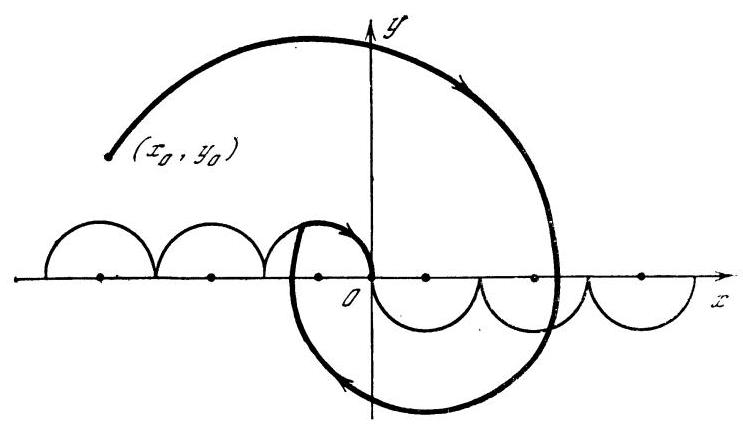
\includegraphics[max width=0.7\textwidth]{images/bo_d547dsv7aajc73fuvc5g_7_561_91_743_425_0.jpg}
\end{center}
\hspace*{3em} 

Система уравнений (9) описывает движение управляемого объекта, где и есть управляющий параметр.

Постараемся теперь привести точку, находящуюся в начальный момент вре- мени в произвольном положении \(\left( {{x}_{0},{y}_{0}}\right)\),в состояние покоя, т. е. в начало ко- ординат фазовой плоскости, за минимальное время, используя для этого уп- равляющий параметр и. Из принципа максимума непосредственно следует, что оптимальное управление и может принимать только значения ±1. При и= = +1 фазовой траекторией системы (9) является окружность с центром в точке (1,0), а при и == — фазовой траекторией системы (9) является окружность c центром в точке (—1,0). Зная, что оптимальное значение и = ±1, мы долж- ны теперь только указать, как меняется \(u\) между этими двумя значениями в процессе движения. Из принципа максимума легко вывести, что значение и зависит лишь от положения фазовой точки на фазовой плоскости, а именно вся фазовая плоскость разбивается на две части, в одной из которых и должно иметь значение +1, а в другой — значение —1. Разбиение фазовой плоскости на две части осуществляется линией, начерченной на рисунке. Она состоит из полу- окружностей радиуса единица, опирающихся как на диаметры на отрезки оси абсцисс. Причем на положительной части абсциссы полуокружности обращены вниз, а на отрицательной части абсциссы полуокружности обращены вверх. Две полуокружности, примыкающие к началу координат, сами являются оп- тимальными траекториями, так что если начальная точка находится на одной из них, то движение в начало координат осуществляется по соответствующей полуокружности. Оказывается дальше, что если фазовая точка находится под. начерченной линией раздела, то и должно иметь значение +1, а если над ли- нией раздела, то значение и должно быть равно —1. Легко вычертить траекто- рию оптимального движения точки (см. рисунок), исходя из произвольного на- чального положения \(\left( {{x}_{0},{y}_{0}}\right)\). Начиная с какой-либо точки плоскости \(\left( {{x}_{0},{y}_{0}}\right)\), движение определяется уравнением (9) с определенным значением и =±1, причем значение это переключается на противоположное, когда соответствую- щая траектория доходит до линии раздела переключения. В конце концов точ- ка попадает на одну из полуокружностей линии раздела, примыкающих к на- чалу координат, после чего точка движется по соответствующей полуокруж- ности к началу координат.

5. Дифференциальные игры. Принцип максимума является всеобъемлющим универсальным методом для решения задач оптимизации. Он нашел многочис- -ленные применения в различных областях знания и оказал существенное влия- ние на развитие вариационного исчисления. В игровых задачах достигнуть ре- зультатов столь общего характера нам не удалось. Ими занимается сейчас боль- шое число математиков, среди которых следует отметить группу сотрудников Математического института им. В. А. Стеклова и школу академика Н. Н. Кра- совского в Свердловске. Ими достигнуты значительные результаты. Здесь я ограничусь тем, что приведу два конкретных примера задачи преследования.

I. В пространстве R произвольной размерности n, где n ≫2, рассмотрим две точки х и у, каждую из которых мы можем одновременно трактовать как вектор. Точку х будем считать преследующей точкой, а точку у — убегающей точкой. Процесс преследования считается законченным, когда х совпадает с у. Движение этих точек описывается следующими уравнениями:

\[
\ddot{x} + \alpha \dot{x} = u,\;\ddot{y} + \beta \dot{y} = v. \tag{10}
\]

Здесь \(u\) и \(v\) — векторы пространства R. В нашей задаче они являются управ- ляющими векторами. Их можно выбирать произвольными по направлению, но они ограничены по длине, а именно для них выполнены условия: | и | < ρ, \(\left| v\right|  \leq  \sigma\). Числа α, β, ρ, σ положительные. Таким образом, уравнение (10) описывает движение точки с линейным трением а под действием внешней силы и, которая может быть выбрана произвольной по направлению, но не превос- ходит по величине числа ρ. Аналогичное верно и для точки у. Процесс пресле- дования можно рассматривать с двух точек зрения. При первой точке зрения мы отождествляем себя с преследователем. Наша задача заключается тогда в за- вершении преследования путем выбора надлежащего управления и. При этом в процессе преследования мы все время наблюдаем за поведением уходящего объекта. При второй точке зрения мы отождествляем себя с убегающим объек- том, и наша задача состоит в том, чтобы уйти от преследования, выбирая надлежащим образом управление v. При этом мы все время наблюдаем за пре- следующим нас объектом. Основной результат, имеющийся здесь, следующий: 1) задача преследования всегда может быть решена положительно, т. е. пре- следование завершено, если выполнены два неравенства

\[
\rho /\alpha  > \sigma /\beta,\;\rho  > \sigma ; \tag{11}
\]

2) задача убегания имеет всегда положительное решение, если выполнено не- равенство σ \(> \rho\).

Оказывается, что при решении задачи преследования в случае, когда вы- полнены условия (11), мы всегда имеем наилучший способ поведения преследо- вания,т. е. имеется единственное оптимальное управление преследователя и (t), отклонение от которого неизбежно увеличивает время преследования. При этом оптимальное управление преследователя и (t) определяется постепенно с возрастанием времени t в зависимости от поведения убегающего объекта.

II. В пространстве R произвольной размерности n ≥2 движение пресле- дующей точки х и убегающей точки у описывается следующими уравнениями:

\[
\ddot{x} = u,\;\left| u\right|  \leq  1;
\]

\[
\dot{y} = v,\;\left| v\right|  \leq  1.
\]

Этот пример был предложен Д. В. Аносовым, который назвал точку хромо- дилом, а точку у — мальчиком. Интуитивно ясно, что задача убегания в этой игре должна решаться положительно. Позже это было выведено из одного на- шего совместного с Е.Ф. Мищенко результата.

\section*{2. Оптимальные процессы регулирования}

Здесь я излагаю результаты, полученные моими учениками В. Г. Болтян- ским и Р. В. Гамкрелидзе и мною [1, 2, 3].

1. Постановка задачи. Пусть Ω — некоторое топологическое пространство. Будем говорить, что задан управляемый процесс, если имеется система обык- новенных дифференциальных уравнений

\[
{\dot{x}}^{i} = {f}^{i}\left( {{x}^{1},{x}^{2},\ldots,{x}^{n},u}\right)  = {f}^{i}\left( {\bar{x},u}\right), \tag{1}
\]

или в векторной форме

\[
\dot{\bar{x}} = \bar{f}\left( {\bar{x},u}\right), \tag{2}
\]

где точкой обозначено дифференцирование по времени, \({x}^{1},\ldots,{x}^{n}\) — действи тельные функции времени t; \(\bar{x} = \left( {{x}^{1},\ldots,{x}^{n}}\right)\) — вектор n-мерного векторного пространства \({R}^{n},u \in  \Omega\), a

\[
{f}^{i}\left( {\bar{x},u}\right) \;\left( {i = 1,\ldots,n}\right)
\]

— функции, заданные и непрерывные для всех значений пары (х, и) ∈ \({R}^{n} \times \; \times  \Omega\). Предполагается также, что частные производные

\[
\frac{\partial {f}^{i}}{\partial {x}^{j}}\;\left( {i,j = 1,\ldots,n}\right)
\]

также определены и непрерывны на всем пространстве R \({}^{n} \times  \Omega\).

Для того чтобы найти решение уравнения (2), определенное на отрезке \({t}_{0} \leq  t \leq  {t}_{1}\),достаточно указать функцию \(u\left( t\right)\) управления на отрезке \(\leq  {t}_{1}\) и начальное значение хор решения при \(t = {t}_{0}\). В соответствии с этим мы бу- дем говорить, что задано управление

\[
U = \left( {u\left( t\right),{t}_{0},{t}_{1},{\bar{x}}_{0}}\right) \tag{3}
\]

уравнения (2), если задана функция \(u\left( t\right)\), отрезок б, с < ≤ <… compeделения и начальное значение х, решения х (t). В дальнейшем будут рассматриваться кусочно-непрерывные функции управления \(u\left( t\right)\),допускающие разрывы перво- ro рода, и непрерывные решения уравнения (2). При этом управления и (1) будут предполагаться непрерывными в начальной точке \({t}_{0}\) и полунепрерывными слева,т. е. удовлетворяющими условию \(u\left( {t - 0}\right)  = u\left( t\right),t > {t}_{0}\). Мы будем го- ворить, что управление (3) переводит точку х, в точку х, если соответствующее решение \(\bar{x}\left( t\right)\) уравнения (2), yдовлетворяющее начальному условию х (и) и удовлетворяет еще конечному условию: \(\bar{x}\left( {t}_{1}\right)  = {x}_{1}\).

Пусть теперь \({f}^{0}\left( {{x}^{1},\ldots,{x}^{n},u}\right)  = {f}^{0}\left( {\bar{x},u}\right)  - \phi\) ункция, определенная и не- прерывная вместе со своими частными производными

\[
\frac{\partial {f}^{0}}{\partial {x}^{j}}\;\left( {j = 1,\ldots,n}\right)
\]

на всем пространстве R" × Ω. Каждому управлению (3) соответствует тогда число

\[
L\left( U\right)  = {\int }_{{t}_{0}}^{{t}_{1}}{f}^{0}\left( {\bar{x}\left( t\right),u\left( t\right) }\right) {dt}.
\]

Таким образом, L есть функционал управления (3). Управление будем называть оптимальным, если, каково бы ни было управление

\[
{U}^{ * } = \left( {{u}^{ * }\left( t\right),{t}_{0}^{ * },{t}_{1}^{ * },{\bar{x}}_{0}}\right),
\]

переводяпее точку \({\bar{x}}_{0}\) в точку \({\bar{x}}_{1}\),имеет место неравенство

\[
L\left( U\right)  \leq  L\left( {U}^{ * }\right).
\]

3 а мечан и е 1. Если (3) — оптимальное управление уравнения (2), пе- реводящее точку \({\bar{x}}_{0}\) в точку \({\bar{x}}_{1}\), a \(\tau  -\) произвольное число,то

\[
{U}^{\prime } = \left( {u\left( {t - \tau }\right),{t}_{0} + \tau,{t}_{1} + \tau,{\bar{x}}_{0}}\right)
\]

— также оптимальное управление, переводящее точку \({\bar{x}}_{0}\) в \({\bar{x}}_{1}\).

3 амечани не 2. Если (3) — оптимальное управление уравнения (2), \(\bar{x}\left( t\right)\) - соответствующее ему решение уравнения (2), a \({t}_{2} < {t}_{3}\) — две точки от- peзка \({t}_{0} \leq  t \leq  {t}_{1}\), то \({U}^{\prime \prime } = \left( {u\left( t\right),{t}_{2},{t}_{3},\bar{x}\left( {t}_{2}\right) }\right)\) ecть также оптимальное управле- ние,переводящее точку \(\bar{x}\left( {t}_{2}\right)\) в точку \(\bar{x}\left( {t}_{3}\right)\).

Важным частным случаем является тот, когда функция \({f}^{0}\left( {\bar{x},u}\right)\) определя- ется равенством

\[
{f}^{0}\left( {\bar{x},u}\right)  \equiv  1. \tag{4}
\]

B этом случае имеем

\[
L\left( U\right)  = {t}_{1} - {t}_{0},
\]

и оптимальность управления U означает минимальность времени перехода из положения \({\bar{x}}_{0}\) в положение \({\bar{x}}_{1}\).

В применениях важен случай, когда Ω является компактным подмножеством некоторого r-мерного евклидова пространства E; тогда и = (и',.., иг) и один управляющий параметр и превращается в систему числовых параметров \({u}^{1}\),..., \({u}^{r}\). В случае, когда Ω представляет собой открытое множество пространст- ва E, сформулированная здесь вариационная задача является частным случаем задачи Лагранжа ([4, с. 225] и основной результат, приводимый ниже (прин- цип максимума), совпадает с известным критерием Вейерштрасса. Для прило- жений важен, однако, случай, когда управляющие параметры удовлетворяют неравенствам, включающим равенства, например

\[
\left| {u}^{i}\right|  \leq  1\;\left( {i = 1,\ldots,r}\right).
\]

В этом случае критерий Вейерштрасса, очевидно, неверен, и приводимый ниже результат является новым.

2. Необходимые условия оптимальности (принцип максимума). Для форму- лировки необходимого условия оптимальности введем в рассмотрение вектор

\[
\widetilde{x} = \left( {{x}^{0},{x}^{\mathrm{T}},\ldots,{x}^{n}}\right)
\]

\(\left( {n + 1}\right)\) -мерного евклидова пространства \({S}^{n + 1}\) и рассмотрим управляемый про- цесс

\[
{\dot{x}}^{i} = {f}^{i}\left( {{x}^{1},\ldots,{x}^{n},u}\right)  = {f}^{i}\left( {\bar{x},u}\right)  = {f}^{i}\left( {\widetilde{x},u}\right), \tag{5}
\]

или в векторной форме

\[
\dot{\widetilde{x}} = \widetilde{f}\left( {\widetilde{x},u}\right), \tag{6}
\]

где \({f}^{0}\left( {\bar{x},u}\right)\) ecть функция, которая определяет функционал \(L\). Для того чтобы, зная управление (3) уравнения (2), получить управление уравнения (6), доста- точно исходя из начального значения

\[
{\bar{x}}_{0} = \left( {{x}_{0}^{1},\ldots,{x}_{0}^{n}}\right)
\]

задатьноезначение \({\widetilde{x}}_{0}\) уравнения \(\left( 6\right)\). Мы определим вектор \({\widetilde{x}}_{0}\),положив

\[
{\widetilde{x}}_{0} = \left( {0,{x}_{0}^{1},\ldots,{x}_{0}^{n}}\right).
\]

Этим способом управление (3) уравнения (2) однозначно определяет управле- ние уравнения (6), и мы просто будем считать, что (3) есть управление уравне- ния (6). Если теперь управление (3) переводит начальное значение ў (6) в конечное значение

\[
{\widetilde{x}}_{1} = \left( {{x}_{1}^{0},{x}_{1}^{1},\ldots,{x}_{1}^{n}}\right),
\]

TO Mbl MMeeM

\[
L\left( U\right)  = {x}_{1}^{0},
\]

и этим определяется связь уравнения (6) с формулированной ранее вариацион- ной задачей.

Наряду с контравариантным вектором ў пространства S\textasciicircum +1 рассмотрим вспо- могательный ковариантный вектор

\[
\widetilde{\psi } = \left( {{\psi }_{0},\ldots,{\psi }_{n}}\right)
\]

этого пространства и составим функцию

\[
K\left( {\widetilde{\psi },\widetilde{x},u}\right)  = \left( {\widetilde{\psi },\widetilde{f}\left( {\widetilde{x},u}\right) }\right)
\]

(справа стоит скалярное произведение векторов Ф и f).

При фиксированных значениях Ф и х функция \(K\) становится функцией па- раметра и; верхнюю грань значений этой функции обозначим через N ( Составим, далее, гамильтонову систему уравнений:

\[
{\dot{x}}^{i} = \frac{\partial K}{\partial {\psi }_{i}}\;\left( {i = 0,\ldots,n}\right) ; \tag{7}
\]

\[
{\dot{\psi }}_{i} =  - \frac{\partial K}{\partial {x}^{i}}\;\left( {i = 0,\ldots,n}\right). \tag{8}
\]

Непосредственно видно, что система (7) совпадает с системой (5), система же (8) есть

\[
{\dot{\psi }}_{0} = 0,\;{\dot{\psi }}_{j} =  - \mathop{\sum }\limits_{{i = 0}}^{n}{\psi }_{i}\frac{\partial {f}^{i}\left( {\widetilde{x},u}\right) }{\partial {x}^{j}}\;\left( {j = 1,\ldots,n}\right). \tag{9}
\]

T e o p e м a 1. Пусть (3) — оптимальное управление уравнения (2) и х (t) — соответствующее ему решение уравнения (2). Дополним вектор х (t) до вектора х \(\widetilde{x}\left( t\right)\), noложив

\[
{x}^{0}\left( t\right)  = {\int }_{{t}_{0}}^{t}{f}^{0}\left( {\bar{x}\left( t\right),u\left( t\right) }\right) {dt}.
\]

Cyuyecmeyem moz∂a makaz nenynegaz Henpepbi6Haz bermop-Hyura WD \(\widetilde{\psi }\left( t\right)\), umo

\[
K\left( {\widetilde{\psi }\left( {t}_{0}\right),\widetilde{x}\left( {t}_{0}\right),u\left( {t}_{0}\right) }\right)  = 0,\;{\psi }_{0}\left( {t}_{0}\right)  \leq  0, \tag{10}
\]

а функции

\[
\widetilde{\psi }\left( t\right),\widetilde{x}\left( t\right),u\left( t\right)
\]

cocmagnatom peuterue zamunbmobooǔ cucmembl (7), (8), npure-m

\[
K\left( {\widetilde{\psi }\left( t\right),\widetilde{x}\left( t\right),u\left( t\right) }\right)  = N\left( {\widetilde{\psi }\left( t\right),\widetilde{x}\left( t\right) }\right) ; \tag{11}
\]

при этом оказывается, что

\[
K\left( {\widetilde{\psi }\left( t\right),\widetilde{x}\left( t\right),u\left( t\right) }\right)  \equiv  0. \tag{12}
\]

Решение ў ( ), (✩ () системы (7), (8), удовлетворяющее условиям (11), (12), будем называть экстремальным, а соответствующую этому решению траекто- рию \(\widetilde{x}\left( t\right)\) — экстремальной.

Для формулировки необходимого условия в случае, когда речь идет о мини- мизации времени (см. (4)), составим гамильтонову функцию

\[
H\left( {\overline{\psi },\bar{x},u}\right)  = \left( {\overline{\psi },\bar{f}\left( {\bar{x},u}\right) }\right).
\]

При фиксированных значениях \(\overline{\psi }\) и \(\bar{x}\) функция \(H\left( {\overline{\psi },\bar{x},u}\right)\) становится функцией параметра и. Верхнюю грань значений этой функции обозначим через М (ψ, 袤). Составим, далее, гамильтонову систему

\[
{\dot{x}}^{j} = \frac{\partial H}{\partial {\psi }_{j}}\;\left( {j = 1,\ldots,n}\right), \tag{13}
\]

\[
{\dot{\psi }}_{j} =  - \frac{\partial H}{\partial {x}^{j}}\;\left( {j = 1,\ldots,n}\right). \tag{14}
\]

Очевидно, что система (13) совпадает с системой (1), а система (14) есть

\[
{\dot{\psi }}_{i} =  - \mathop{\sum }\limits_{{j = 1}}^{n}{\psi }_{j}\frac{\partial {f}^{j}\left( {\bar{x},u}\right) }{\partial {x}^{i}}\;\left( {i = 1,\ldots,n}\right). \tag{15}
\]

Теорема 2. Пусть (3) — оптимальное для функционала (4) управления уравнения (2) и ā (t) — соответствующее этому управлению решение уравнение (2). Существует тогда такая ненулевая непрерывная вектор-функция \(\overline{\psi }\left( t\right)  = \; = \left( {{\psi }_{1}\left( t\right),\ldots,{\psi }_{n}\left( t\right) }\right),\) что

\[
H\left( {\overline{\psi }\left( {t}_{0}\right),\bar{x}\left( {t}_{0}\right),u\left( {t}_{0}\right) }\right)  \geq  0,
\]

a 釣りHKYUU

\[
\overline{\psi }\left( t\right),\bar{x}\left( t\right),u\left( t\right)
\]

убовдемворяюм еамцльмоновой ссгененцй (13), (14), причем

\[
H\left( {\overline{\varphi }\left( t\right),\bar{x}\left( t\right),u\left( t\right) }\right)  = M\left( {\overline{\psi }\left( t\right),\bar{x}\left( t\right) }\right). \tag{16}
\]

Оказывается, кроме того, что функция H (ψ (t), x (t)) постоянна, так что

\[
H\left( {\overline{\psi }\left( t\right),\bar{x}\left( t\right),u\left( t\right) }\right)  \geq  0. \tag{17}
\]

Теорема 2 непосредственно вытекает из теоремы 1.

Главным содержанием теорем 1 и 2 являются равенства (11) и (16). Поэто- му теорема 2, первоначально опубликованная в качестве гипотезы в заметке [1], названа принципом максимума. В этом же смысле и теореме 1 естественно присвоить наименование принципа максимума.

3. Доказательство принципа максимума (теоремы 1 и 2). Докажем теорему 1. В доказательстве использованы вариации Макшейна [5]. Пусть (3) — некоторое управление уравнения (6) и ў (t) — соответствующее ему решение уравнения (6). Система уравнений в вариациях для системы (5) вдоль решения ў (t) запи- сывается, как известно, в виде

\[
{\dot{y}}^{i} = \mathop{\sum }\limits_{{j = 0}}^{n}\frac{\partial {f}^{i}\left( {\widetilde{x}\left( t\right),u\left( t\right) }\right) }{\partial {x}^{j}}{y}^{j}\;\left( {i = 0,1,\ldots,n}\right). \tag{18}
\]

Записывая решение системы (18) в векторной форме, получаем вектор

\[
\widetilde{y}\left( t\right)  = \left( {{y}^{0}\left( t\right),\ldots,{y}^{n}\left( t\right) }\right).
\]

В дальнейшем будут рассматриваться только непрерывные решения ў (). Си- стему уравнений в вариациях, как известно, можно истолковать следующим об- разом. Пусть \({\widetilde{y}}_{0}\) — произвольный вектор пространства S\textasciicircum 1- Зададимся началь- ным значением

\[
{\widetilde{x}}_{0} + \varepsilon {\widetilde{y}}_{0} + {\varepsilon O}\left( \varepsilon \right)
\]

для решения уравнения (6). Тогда само решение уравнения (6) с этим началь- ным значением записывается в форме

\[
\widetilde{x}\left( t\right)  + \varepsilon \widetilde{y}\left( t\right)  + {\varepsilon O}\left( \varepsilon \right), \tag{19}
\]

где \(\widetilde{y}\left( t\right)\) есть решение системы (18),взятое с начальным значением \({\widetilde{y}}_{0}\). Мы будем товорить, что решение ў (t) системы (18) является перенесением вектора ўу, заданного в начальной точке \({\widetilde{x}}_{0}\) траектории \(\widetilde{x}\left( t\right)\),вдоль всей траектории. В том же смысле можно сказать, что решение ў (н) является перенесением вектора \(\widetilde{y}\left( \tau \right)\),заданного в точке ў (т) траектории \(\widetilde{x}\left( t\right)\),вдоль всей траектории.

Наряду с контравариантным вектором ў (t), являющимся решением системы (18), рассмотрим ковариантный вектор \(\widetilde{\psi }\left( t\right)\), являющийся решением системы (8). Непосредственно проверяется, что

\[
\frac{d}{dt}\left( {\widetilde{\psi }\left( t\right),\widetilde{y}\left( t\right) }\right)  = 0,
\]

TAK YTO

\[
\left( {\widetilde{\psi }\left( t\right),\widetilde{y}\left( t\right) }\right)  = \text{ const. }
\]

Если истолковывать ковариантный вектор ф (t) как ориентированную плос- кость, проведенную через точку \(\widetilde{x}\left( t\right)\), то можно сказать, что плоскость \(\widetilde{\psi }\left( t\right)\) яв- ляется перенесением плоскости \(\widetilde{\psi }\left( \tau \right)\),заданной в точке ў (т) траектории ё (н), вдоль всей траектории.

Вариацией управления (3) будем называть управление

\[
{U}^{ * } = {U}^{ * }\left( {\varepsilon,\alpha }\right)  = \left( {{u}^{ * }\left( t\right),{t}_{0},{t}_{1} + {\alpha \varepsilon },{\widetilde{x}}_{0}}\right),
\]

зависящее от параметра в и действительного числа α, определенное для всех достаточно малых положительных значений параметра ε и удовлетворяющее следующему условию:

Решение 8* уравнения (6), соответствующее управлению \({U}^{ * }\), в точке t = \(= {t}_{1} + {\varepsilon \alpha }\) может быть записано в виде

\[
\widetilde{x}\left( {t}_{1}\right)  + \varepsilon \widetilde{\delta }\left( {U}^{ * }\right)  + {\varepsilon O}\left( \varepsilon \right),
\]

где б \(\left( {U}^{ * }\right)\) не зависит от ε.

Семейство ∆ вариаций одного и того же управления (3) будем называть до- пустимым, если наряду с каждыми двумя вариациями \({U}_{1}^{ * }\left( {\varepsilon,{\alpha }_{1}}\right)\) и \({U}_{2}^{ * }\left( {\varepsilon,{\alpha }_{2}}\right)\) в нем найдется при любых неотрицательных \({\gamma }_{1},{\gamma }_{2}\) третья вариация \({U}^{ * }\) (ε, \(\left. {{\gamma }_{1}{\alpha }_{1} + {\gamma }_{2}{\alpha }_{2}}\right)\), yдовлетворяющая условию

\[
\widetilde{\delta }\left( {U}^{ * }\right)  = {\gamma }_{1}\widetilde{\delta }\left( {U}_{1}^{ * }\right)  + {\gamma }_{2}\widetilde{\delta }\left( {U}_{2}^{ * }\right). \tag{20}
\]

Опишем теперь вариацию Макшейна

\[
{U}^{ * }\left( {\varepsilon,\alpha }\right)  = V\left( {\varepsilon,\alpha,\tau,\sigma,{u}^{ * }}\right),
\]

зависящую от точки τ полуинтервала \({t}_{0} < t \leq  {t}_{1}\) (причем при а < 0 должно быть \(\tau  < {t}_{1}\) ),неотрицательного числа σ и точки и* пространства Ω. Вариацию \(V\left( {\varepsilon,\alpha,\tau,\sigma,{u}^{ * }}\right)\) omределим,задав Šункцию \({u}^{ * }\left( t\right)\) соотношениями

\[
{u}^{ * }\left( t\right)  = \left\{  \begin{array}{ll} u\left( t\right) & \text{ при }{t}_{0} \leq  t \leq  \tau  - {\varepsilon \sigma }, \\  {u}^{ * } & \text{ при }\tau  - {\varepsilon \sigma } < t \leq  \tau, \\  u\left( t\right) & \text{ при }\tau  < t \leq  {t}_{1}, \\  u\left( {t}_{1}\right) & \text{ при }{t}_{1} < t \leq  {t}_{1} + {\varepsilon \alpha }\left( {\operatorname{\text{ е }\text{ с }\text{ л }\text{ и }}\alpha  > 0}\right). \end{array}\right. \tag{21}
\]

Легко построить допустимое семейство ∆, содержащее все вариации Макшейна. Это семейство ∆ и будет положено в основу дальнейших построений.

Каждой вариации \({U}^{ * }\) допустимого семейства ∆ соответствует вектор Õ \(\left( {U}^{ * }\right)\), выходящий из точки ёх. Совокупность всех этих векторов заполняет выпуклый конус (см. (20)) \(\Pi\) c вершиной в точке \({\widetilde{x}}_{1}\). Пусть

\[
\widetilde{v} = \left( {-1,0,\ldots,0}\right)
\]

— вектор, выходящий из точки ёх и идущий в направлении отрицательной оси \({x}^{0}\) в пространстве S"+. Если конус П содержит конец вектора ё в качестве внут- ренней точки, то управление И не является оптимальным. Пусть, в самом деле, \({U}^{ * } \in  \Omega  -\) ta вариация управления \(U\),для которой

\[
\widetilde{\delta }\left( {U}^{ * }\right)  = \widetilde{v}.
\]

Обозначая через хз точку, в которую переходит точка х, при управлении U*, получаем

\[
{\widetilde{x}}_{1}^{ * } = {\widetilde{x}}_{1} + \varepsilon \widetilde{v} + {\varepsilon O}\left( \varepsilon \right).
\]

Расщепляя это равенство на скалярное для нулевой координаты и векторное для остальных координат, получаем

\[
L\left( {U}^{ * }\right)  = {x}_{1}^{0 * } = {x}_{1}^{0} - \varepsilon  + {\varepsilon O}\left( \varepsilon \right)  = L\left( U\right)  - \varepsilon  + {\varepsilon O}\left( \varepsilon \right),
\]

\[
{\bar{x}}_{1}^{ * } = {\bar{x}}_{1} + {\varepsilon O}\left( \varepsilon \right)
\]

Таким образом, функционал уменьшен на величину порядка ε, а конец тра- ектории отличается от желательного на величину вО(в). Уточнение этого по- строения приводит нас к такой вариации \({U}^{ * } \in  \Delta\),для которой конец ў тории \(\widetilde{x}\) \# удовлетворяет точному равенству ў \({\widetilde{x}}_{1}^{\# } = {\widetilde{x}}_{1} + \varepsilon \widetilde{v}\), a это противоречит предположению об оптимальности управления U.

Итак, предполагая, что управление U оптимально, мы будем считать в даль- нейшем, что вектор \(\widetilde{v}\) не является внутренним для конуса П. Так как конус П выпуклый, то для него существует такая опорная плоскость Г, что сам конус лежит в одном полупространстве (замкнутом), определяемом этой плоскостью, а вектор \(\widetilde{v} -\) в другом. Обозначая через \({\widetilde{\psi }}_{1}\) ковариантный вектор, coответствую- щий плоскости \(\Gamma\),выбранный с надлежащим знаком,мы получаем

\[
\left( {{\widetilde{\psi }}_{1},\widetilde{\delta }\left( {U}^{ * }\right) }\right)  \leq  0\;\left( {{U}^{ * } \in  \Delta }\right), \tag{22}
\]

\[
\left( {{\psi }_{1},\widetilde{v}}\right)  \geq  0\text{. } \tag{23}
\]

Из неравенства (23) сразу следует неравенство

\[
{\psi }_{1,0} \leq  0\text{. } \tag{24}
\]

Обозначим через у вектора \({\widetilde{\psi }}_{1}\),заданного в точке ёх, вдоль всей траектории ёх (не обе мексем ем успевк- тор-функция \(\widetilde{\psi }\left( t\right)\) и есть та, существование которой утверждается в теореме 1.

Пусть \(V\left( {\varepsilon,0,\tau,\sigma,{u}^{ * }}\right)\) — произвольная вариация Макшейна (см. (21)) ce- мейства ∆ и ++ (+) – соответствующее ей решение уравнения (6). Простые

BEITICICHINA ARIOT

\[
{\widetilde{x}}^{ * }\left( \tau \right)  = \widetilde{x}\left( \tau \right)  + \varepsilon \left\lbrack  {\widetilde{f}\left( {\widetilde{x}\left( \tau \right),{u}^{ * }}\right)  - \widetilde{f}\left( {\widetilde{x}\left( \tau \right),u\left( \tau \right) }\right) }\right\rbrack   + {\varepsilon O}\left( \varepsilon \right).
\]

Обозначим через \(\widetilde{y}\left( t\right)\) вектор,получающийся из вектора

\[
\widetilde{y}\left( \tau \right)  = \widetilde{f}\left( {\widetilde{x}\left( \tau \right),{u}^{ * }}\right)  - \widetilde{f}\left( {\widetilde{x}\left( \tau \right),u\left( \tau \right) }\right),
\]

заданноговточке \(\widetilde{x}\left( \tau \right)\),путем переносавдольтраектории \(\widetilde{x}\left( t\right)\).Тогдмы имеем

\[
{\widetilde{x}}^{ * }\left( {t}_{1}\right)  = {\widetilde{x}}_{1} + \varepsilon \widetilde{y}\left( {t}_{1}\right)  + {\varepsilon O}\left( \varepsilon \right).
\]

Так как вектор \(\widetilde{y}\left( {t}_{1}\right)\) принадлежит конусу П, то в силу неравенства (22) полу- чаем

\[
\left( {\widetilde{{\psi }_{1}},\widetilde{y}\left( {t}_{1}\right) }\right)  \leq  0
\]

B силу (19) отсюда получаем

\[
\left( {\widetilde{\psi }\left( \tau \right),\widetilde{f}\left( {\widetilde{x}\left( \tau \right),{u}^{ * }}\right)  - \widetilde{f}\left( {\widetilde{x}\left( \tau \right),u\left( \tau \right) }\right) }\right)  \leq  0.
\]

Переписывая последнее неравенство в обозначениях функции \(K\),получаем не- равенство

\[
K\left( {\widetilde{\psi }\left( \tau \right),\widetilde{x}\left( \tau \right),u\left( \tau \right) }\right)  \geq  K\left( {\widetilde{\psi }\left( \tau \right),\widetilde{x}\left( \tau \right),{u}^{ * }}\right),
\]

эквивалентное равенству (11).

Пусть теперь U* = V ( s, α, τ, 0, u*). Решение уравнения (6), соответствую- щее этому управлению U*, обозначим через х* (t). Мы имеем, очевидно,

\[
{\widetilde{x}}^{ * }\left( {{t}_{1} + {\alpha \varepsilon }}\right)  = {\widetilde{x}}_{1} + \varepsilon \widetilde{\delta }\left( {U}^{ * }\right)  + {\varepsilon O}\left( \varepsilon \right),
\]

где

\[
\widetilde{\delta }\left( {U}^{ * }\right)  = \alpha \widetilde{f}\left( {{\widetilde{x}}_{1},u\left( {t}_{1}\right) }\right).
\]

Так как вектор \(\widetilde{\delta }\left( {U}^{ * }\right)\) принадлежит конусу П, то в силу неравенства (22) по лучаем

\[
\alpha \left( {{\widetilde{\psi }}_{1},\widetilde{f}\left( {{\widetilde{x}}_{1},u\left( {t}_{1}\right) }\right) }\right)  \leq  0.
\]

Ввиду того что α есть произвольное действительное число, последнее неравен- ство возможно лишь при условии

\[
\left( {{\widetilde{\psi }}_{1},\widetilde{f}\left( {{\widetilde{x}}_{1},u\left( {t}_{1}\right) }\right) }\right)  = 0,
\]

T. e. при

\[
K\left( {\widetilde{\psi }\left( {t}_{1}\right),\widetilde{x}\left( {t}_{1}\right),u\left( {t}_{1}\right) }\right)  = 0. \tag{25}
\]

Докажем, наконец, что функция \(K\left( t\right)  = K\left( {\widetilde{\psi }\left( t\right),\widetilde{x}\left( t\right),u\left( t\right) }\right)\) переменного \(t\) постоянна. Пусть \({t}_{0} \leq  {t}_{2} < {t}_{3} \leq  {t}_{1}\),причем на полуинтервале \({t}_{2} < t \leq  {t}_{3}\) функ- ция \(u\left( t\right)\) непрерывна. Покажем,что на этом полуинтервале функция \(K\left( t\right)\) поc- тоянна. Возьмем две произвольные точки \({\tau }_{0}\) и \({\tau }_{1}\) полуинтервала \({t}_{2} < t \leq  {t}_{3}\). B силу (11) имеем

\[
K\left( {\widetilde{\psi }\left( {\tau }_{0}\right),\widetilde{x}\left( {\tau }_{0}\right),u\left( {\tau }_{0}\right) }\right)  - K\left( {\widetilde{\psi }\left( {\tau }_{0}\right),\widetilde{x}\left( {\tau }_{0}\right),u\left( {\tau }_{1}\right) }\right)  \geq  0,
\]

\[
- K\left( {\widetilde{\psi }\left( {\tau }_{1}\right),\widetilde{x}\left( {\tau }_{1}\right),u\left( {\tau }_{1}\right) }\right)  + K\left( {\widetilde{\psi }\left( {\tau }_{1}\right),\widetilde{x}\left( {\tau }_{1}\right),u\left( {\tau }_{0}\right) }\right)  \leq  0.
\]

Прибавляя к обеим частям этих неравенств разность \(K\left( {\tau }_{1}\right)  - K\left( {\tau }_{0}\right)\),полу- чим неравенства

\[
- K\left( {\widetilde{\psi }\left( {\tau }_{0}\right),\widetilde{x}\left( {\tau }_{0}\right),u\left( {\tau }_{0}\right) }\right)  + K\left( {\widetilde{\psi }\left( {\tau }_{1}\right),\widetilde{x}\left( {\tau }_{1}\right),u\left( {\tau }_{0}\right) }\right)  \leq  K\left( {\tau }_{1}\right)  - K\left( {\tau }_{0}\right)  \leq
\]

\[
\leq  K\left( {\widetilde{\psi }\left( {\tau }_{1}\right),\widetilde{x}\left( {\tau }_{1}\right),u\left( {\tau }_{1}\right) }\right)  - K\left( {\widetilde{\psi }\left( {\tau }_{0}\right),\widetilde{x}\left( {\tau }_{0}\right),u\left( {\tau }_{1}\right) }\right). \tag{26}
\]

Наряду с системой (7), (8) рассмотрим аналогичную систему уравнений. Для того чтобы выявить более четко разницу между двумя этими системами, запиппем систему (7), (8) в более развернутом виде:

\[
{\dot{x}}^{i} = \frac{\partial }{\partial {\psi }_{i}}K\left( {\widetilde{\psi }\left( t\right),\widetilde{x}\left( t\right),u\left( t\right) }\right), \tag{27}
\]

\[
{\dot{\psi }}_{i} =  - \frac{\partial }{\partial {x}^{i}}K\left( {\widetilde{\psi }\left( t\right),\widetilde{x}\left( t\right),u\left( t\right) }\right). \tag{28}
\]

Наряду с этой системой рассмотрим систему

\[
{\dot{x}}_{{\tau }_{0}}^{i} = \frac{\partial }{\partial {\psi }_{i}}K\left( {{\widetilde{\psi }}^{{\tau }_{0}}\left( t\right),{\widetilde{x}}_{{\tau }_{0}}\left( t\right),u\left( {\tau }_{0}\right) }\right), \tag{29}
\]

\[
{\dot{\psi }}_{i}^{{\tau }_{0}} =  - \frac{\partial }{\partial {x}^{i}}K\left( {{\widetilde{\psi }}^{{\tau }_{0}}\left( t\right),{\widetilde{x}}_{{\tau }_{0}}\left( t\right),u\left( {\tau }_{0}\right) }\right) \tag{30}
\]

(индексы то в уравнениях (29), (30) указывают на то, что соответствующие функ- ции суть решение системы (7), (8) при фиксированном и = и (τ0)).

Наряду с векторами х, у введем векторы

\[
\widehat{x}\left( t\right)  = \left( {{x}_{{\tau }_{0}}^{0}\left( t\right),{x}_{{\tau }_{0}}^{1}\left( t\right),\ldots,{x}_{{\tau }_{0}}^{n}\left( t\right) }\right),
\]

\[
\widehat{\psi }\left( t\right)  = \left( {{\psi }_{0}^{{\tau }_{0}}\left( t\right),{\psi }_{1}^{{\tau }_{0}}\left( t\right),\ldots,{\psi }_{n}^{{\tau }_{0}}\left( t\right) }\right).
\]

Мы будем рассматривать функцию \(K\left( {\widehat{\psi }\left( t\right),\widehat{x}\left( t\right),u\left( {\tau }_{0}\right) }\right)\). Из системы (29),(30) следует непосредственно, что

\[
\frac{d}{dt}K\left( {\widehat{\psi }\left( t\right),\widehat{x}\left( t\right),u\left( {\tau }_{0}\right) }\right)  = 0.
\]

Легко показать, что функции \(K\left( {\widetilde{\psi }\left( t\right),\widetilde{x}\left( t\right),u\left( {\tau }_{0}\right) }\right)\) и K \(\left( {\widehat{\psi }\left( t\right),\widehat{x}\left( t\right),u\left( {\tau }_{0}\right) }\right)\) мало отличаются друг от друга, а именно имеет место неравенство

\[
\left| {K\left( {\overline{\psi }\left( t\right),\widetilde{x}\left( t\right),u\left( {\tau }_{0}\right) }\right)  - K\left( {\widehat{\psi }\left( t\right),\widehat{x}\left( t\right),u\left( {\tau }_{0}\right) }\right) }\right|  \leq  \left| {t - {\tau }_{0}}\right| \gamma, \tag{31}
\]

где \(\mathop{\lim }\limits_{{\left| {t - {\tau }_{0}}\right|  \rightarrow  0}}\gamma  = 0\).

Так как функция и (t) непрерывна на рассматриваемом полуинтервале, то решения систем (27), (28) и (29), (30) мало отличаются друг от друга, а именно имеют место неравенства

\[
\left| {\widetilde{x}\left( t\right)  - \widehat{x}\left( t\right) }\right|  \leq  \left| {t - {\tau }_{0}}\right| {\gamma }_{1}, \tag{32}
\]

\[
\left| {\widetilde{\psi }\left( t\right)  - \widehat{\psi }\left( t\right) }\right|  \leq  \left| {t - {\tau }_{0}}\right| {\gamma }_{2}, \tag{33}
\]

где

\[
\mathop{\lim }\limits_{{\left| {t - {\tau }_{0}}\right|  \rightarrow  0}}{\gamma }_{1} = \mathop{\lim }\limits_{{\left| {t - {\tau }_{0}}\right|  \rightarrow  0}}{\gamma }_{2} = 0.
\]

Из неравенств (32), (33) следует неравенство (31). Теперь, пользуясь неравенст- вом (31), мы усилим неравенства (26) следующим образом:

\[
- \left( {{\tau }_{1} - {\tau }_{0}}\right) \gamma  \leq  K\left( {\tau }_{1}\right)  - K\left( {\tau }_{0}\right)  \leq  \left( {{\tau }_{1} - {\tau }_{0}}\right) \gamma.
\]

Деля это неравенство на \({\tau }_{1} - {\tau }_{0}\) и переходя к пределу при | \({\tau }_{1} - {\tau }_{0}\) | \(\rightarrow  0\), no- лучаем окончательный результат

\[
\frac{d}{dt}K\left( t\right)  = 0.
\]

Таким образом, на полуинтервале \({t}_{2} < t \leq  {t}_{3}\) функция \(K\left( t\right)\) постоянна.

Докажем теперь, что функция \(N\left( {\widetilde{\psi },\widetilde{x}}\right)\) непрерывна по паре аргументов \(\widetilde{\psi },\widetilde{x}\). Если это неверно, то существуют такие близкие между собой пары (Ф1, гх) и ( \({\widetilde{\psi }}_{0},{\widetilde{x}}_{0}\) ), что при сколь угодно малом расстоянии между ними имеет место не- равенство

\[
N\left( {{\widetilde{\psi }}_{1},{\widetilde{x}}_{1}}\right)  - N\left( {{\widetilde{\psi }}_{0},{\widetilde{x}}_{0}}\right)  > c > 0.
\]

Пусть \({u}_{1}\) и \({u}_{0}\) 一 такие значения управления \(u\),что

\[
N\left( {{\widetilde{\psi }}_{1},{\widetilde{x}}_{1}}\right)  = K\left( {{\widetilde{\psi }}_{1},{\widetilde{x}}_{1},{u}_{1}}\right),
\]

\[
N\left( {{\widetilde{\psi }}_{0},{\widetilde{x}}_{0}}\right)  = K\left( {{\widetilde{\psi }}_{0},{\widetilde{x}}_{0},{u}_{0}}\right).
\]

Так как идет максимум, то имеет место неравенство

\[
K\left( {{\widetilde{\psi }}_{1},{\widetilde{x}}_{1},{u}_{1}}\right)  - K\left( {{\widetilde{\psi }}_{0},{\widetilde{x}}_{0},{u}_{1}}\right)  > c,
\]

что противоречит непрерывности \(K\) по первым двум аргументам. Отсюда следует непрерывность функции \(K\left( {\widetilde{\psi }\left( t\right),\widetilde{x}\left( t\right),u\left( t\right) }\right)\) и в точке разрыва функции \(u\left( t\right)\).

Из доказанного вытекает (см. (25)) справедливость равенства (12) на всем отрезке \({t}_{0} \leq  t \leq  {t}_{1}\),чем,в частности, доказано первое из соотношений (10). Второе из соотношений (10) следует из неравенства (24) в силу первого уравне- ния (9).

Итак, теорема 1 полностью доказана, а тем самым доказана и теорема 2.

3 амечан и е 3. Если вместо условий х ( \({t}_{0}\) ) = \({\bar{x}}_{0},\bar{x}\left( {t}_{1}\right)  = {\bar{x}}_{1}\) выдвинуты более общие условия

\[
\bar{x}\left( {t}_{0}\right)  \in  {M}_{0},\;\bar{x}\left( {t}_{1}\right)  \in  {M}_{1}, \tag{34}
\]

где \({M}_{0}\) и \({M}_{1}\) — два гладких многообразия произвольных размерностей из \({R}^{n}\), то наряду с условиями (34) возникают условия трансверсальности, а именно типерплоскость \(\psi \left( {t}_{0}\right)\) касается многообразия \({M}_{0}\) в точке \(\bar{x}\left( {t}_{0}\right)\), a runepплоскость \(\overline{\psi }\left( {t}_{1}\right)\) касается многообразия \({M}_{1}\) в точке х (t,) (любое из многообразий и, \({M}_{0}\), \({M}_{1}\) может быть, в частности, точкой).

3 а м е ч а н и е 4. Теорема 1 и замечание 3 остаются верными и в случае, если функции \(u\left( t\right)\) измеримы и ограничены; только равенство (11) выполняется почти всюду.

4. Синтез оптимального по быстродействию управления. Из формулировки принципа максимума (теорема 2), дополненной замечанием 3, видно, что для нахождения оптимальной траектории и оптимального управления необходимо решить краевую задачу для систем обыкновенных дифференциальных уравне- ний, что является непростой задачей. Очень часто задача оптимизации ставится не совсем так, как в теореме 2 и замечании 3, а именно следующим образом.

Известно то многообразие М1, на которое должна придти фазовая точка. В частности, это многообразие \({M}_{1}\) может оказаться просто одной точкой \({\bar{x}}_{1}\), а исходное фазовое состояние \({\bar{x}}_{0}\) считается произвольным. Если мы решим зада- чу оптимизации по быстродействию для исходной точки х, и конечного поло- жения \({M}_{1}\), то в начальный момент \({t}_{0}\) определяется управление \(u\left( {t}_{0}\right)\), соответ- ствующее точке \({\bar{x}}_{0}\) и которое естественно обозначить через и ( \({\bar{x}}_{0}\) ). Поскольку мы хотим считать начальное состояние хоч произвольным, то естественно обоз- начить \({\bar{x}}_{0}\) через \(\bar{x}\),и мы получим тогда \(u\) как функцию \(u\left( \bar{x}\right)\) положения точки в пространстве. Подставим теперь в уравнение, определяющее управляемую сис- тему (3), вместо \(u\dot{\Phi }\) ункцио \(u\left( \bar{x}\right)\). Тогда мы получим систему уравнений

\[
\dot{\bar{x}} = f\left( {\bar{x},u\left( \bar{x}\right) }\right).
\]

Решая эту систему уравнений при начальном условии х биби = х, мы получим экстремальную траекторию, идущую из состояния хв на многообразие \({M}_{1}\). Нахождение управления и (х) как функции точки х пространства, называется синтезом оптимального управления.

Для нахождения синтезирующей функции \(u\left( \bar{x}\right)\) можно использовать тео- рему 2 и замечание 3 следующим образом: на многообразии М1 зададимся произ- вольной точкой \({\bar{x}}_{1}\) и произвольной ориентированной гиперплоскостью \({\overline{\psi }}_{1}\), касающейся многообразия \({M}_{1}\) в точке \({\bar{x}}_{1}\). Исходя из начальных данных \({\bar{x}}_{1}\) и \({\overline{\psi }}_{1}\) при \(t = 0\) будем решать систему уравнений (13),(14),дополненную условием (16) при t, убывающем от 0 до некоторого \({t}_{0} < 0\). В результате этого попятного движения мы придем в положение х = x (t0). Ясно теперь, что, двигаясь из это- го положения при t возрастающем от t, до 0, мы получим экстремальную траек- торию, причем й (0) = 퀸 и выполнено условие трансверсальности на \({M}_{1}\). Точка \(\bar{x}\left( {t}_{0}\right)\) зависит от \({t}_{0}\),которое является отрицательным числом, a также от началь- ных значений \({\bar{x}}_{1},{\overline{\psi }}_{1}\). Таким образом, следует написать

\[
x\left( {t}_{0}\right)  = \omega \left( {{\bar{x}}_{1},{\overline{\psi }}_{1},{t}_{0}}\right).
\]

Если размерность многообразия \({M}_{1}\) равна v, то размерность совокупности всех ориентированных гиперплоскостей, касающихся многообразия \({M}_{1}\) в точке \({\bar{x}}_{1}\), paвна \(n - v - 1\). Так как размерность многообразия \({M}_{1}\) paвна v,то раз- мерность многообразия всех пар (х, т, ч, е, размерность всех возможных на- чальных значений равна л — 1, а функция о зависит еще от одного скалярного параметра \({t}_{0} < 0\). Если обозначить аргумент функции о через ξ,т. е. положить \(\xi  = \left( {{\bar{x}}_{1},{\overline{\psi }}_{1},{t}_{0}}\right)\), to paзмерность многообразия \({S}^{n}\) всех значений ξ равна л. Та- ким образом, ω есть отображение n-мерного многообразия \({S}^{n}\) в евклидово про- странство \({R}^{n}\). При построении экстремальной траектории с начальными зна- чениями \(\left( {{\bar{x}}_{1},{\overline{\psi }}_{1}}\right)\),ведущей в точку х би не всей траектории определяется уп- равление \(u\left( t\right)\). Таким образом, оно определено и при t = t, т. е. в точке йо, так что в этой точке мы нашли синтезирующее управление \(u\left( {\bar{x}}_{0}\right)\),где \({\bar{x}}_{0} = \bar{x}\left( {t}_{0}\right)\). Здесь мы не разбираем вопросов существования и единственности реше- ния, но в некоторых случаях этот способ синтезирования оптимального управ- ления удается. Синтезирующее управление, данное в п. 4 раздела 1, построено именно таким способом.

5. Линейные управляемые системы. Важным для приложений и хорошо иллюстрирующим общие результаты примером является линейная управляе- man cuctema

\[
{\dot{x}}^{i} = \mathop{\sum }\limits_{{j = 1}}^{n}{a}_{j}^{i}{x}^{j} + {u}^{i}\;\left( {i = 1,\ldots,n}\right),
\]

где й = (и*,.., и*) есть точка выпуклого замкнутого ограниченного много- гранника Ω произвольной размерности, расположенного в линейном простран- стве R". В векторном виде эта система может быть записана так:

\[
\dot{\bar{x}} = A\bar{x} + \bar{u}, \tag{35}
\]

где A — линейный оператор в пространстве R \({}^{n}\) переменных \({x}^{\mathrm{I}}\),.., \({x}^{n}\). Мы бу- дем рассматривать здесь только задачу о минимализации функционала \({\int }_{{t}_{0}}^{{t}_{1}}{dt}\), т. е. задачу минимизации времени перехода.

Для получения некоторых результатов характера единственности мы будем налагать на управляемую систему (35) нижеследующие условия (А), (В), роль которых выявится в дальнейшем:

(A) Если и — некоторый вектор, имеющий направление какого-либо из ребер многогранника Ω, то векторы

\[
\bar{w},A\bar{w},\ldots,{A}^{n - 1}\bar{w} \tag{36}
\]

линейно независимы.

(B) Начало координат пространства R" является внутренней точкой мно- гогранника \(\Omega\).

Функция \(H\left( {\psi,\bar{x},u}\right)\) в нашем случае имеет вид

\[
H = \left( {\overline{\psi },A\bar{x}}\right)  + \left( {\overline{\psi },\bar{u}}\right), \tag{37}
\]

а система (15) записывается в виде

\[
{\dot{\psi }}_{j} =  - \mathop{\sum }\limits_{{i = 1}}^{n}{a}_{j}^{i}{\psi }_{i}\;\left( {j = 1,\ldots,n}\right),
\]

или в векторной форме

\[
\dot{\psi } =  - A * \overline{\psi }, \tag{38}
\]

где \({A}^{ * }\) - транспонированная матрица \(A\).

Очевидно, что функция \(H\), рассматриваемая как функция переменного \(\bar{u} \in  \Omega\), достигает максимума одновременно с функцией ( \(\overline{\psi }\), й). В соответствии с этим обозначим через \(P\left( \overline{\psi }\right)\) максимум функции \(\left( {\overline{\psi },\bar{u}}\right)\), paccматриваемой как функция переменного й € Ω. Из теоремы 2 следует, таким образом, что если

\[
U = \left( {\bar{u}\left( t\right),{t}_{0},{t}_{1},{\bar{x}}_{0}}\right)
\]

есть оптимальное управление системы (35), то существует такое решение ф (не уравнения (38), что

\[
\left( {\overline{\psi }\left( t\right),\bar{u}\left( t\right) }\right)  = P\left( {\overline{\psi }\left( t\right) }\right). \tag{39}
\]

Так как уравнение (38) не содержит неизвестных функций \(\bar{x}\left( t\right)\) и ā (t), то все решения уравнения (38) легко могут быть найдены, и тем самым по условию (39) легко могут быть найдены и все оптимальные управления \(\bar{u}\left( t\right)\) системы (35). Вопрос о том, насколько однозначно условие (39) определяет управление и (t) через функцию \(\overline{\psi }\left( t\right)\), peшается нижеследующей теоремой:

T e o p e м a 3. Если выполнено условие (А), то при заданном нетривиальном решении up (t) уравнения (38) соотношение (39) однозначно определяет управляю- щую функцию й (t); при этом оказывается, что функция й (t) кусочно-постоянна и ее значениями являются лишь вершины многогранника Ω.

Доказательство. Так как функция

\[
\left( {\overline{\psi }\left( t\right),\bar{u}}\right) \text{, } \tag{40}
\]

рассматриваемая как функция вектора й, линейна, то она либо постоянна, либо достигает своего максимума на границе многогранника Ω. Это же сооб- ражение применимо и к каждой грани многогранника Ω. Таким образом, либо функция (40) достигает своего максимума лишь в одной вершине многогранника \(\Omega\), либо же достигает его на целой грани многогранника \(\Omega\). Покажем, что в силу условия (А) последнее возможно лишь для конечного числа значений t. Допустим, что функция (40) достигает своего максимума (и, следовательно, пос- тоянна) на некоторой грани Г многогранника Ω. Пусть т вектор, имеющий направление некоторого ребра грани Г. В,силу постоянства функции (40) на грани \(\Gamma\) имеем

\[
\left( {\overline{\psi }\left( t\right),\bar{w}}\right)  = 0.
\]

Если бы это соотношение имело место для бесконечного множества значений переменного \(t\) из отрезка [ \({t}_{0},{t}_{1}\) ], то оно выполнялось бы тождественно по t и, дифференцируя его последовательно по \(t\),мы получили бы

\[
\left( {\overline{\psi }\left( t\right),\bar{w}}\right)  = 0
\]

\[
\left( {{A}^{ * }\overline{\psi }\left( t\right),\bar{w}}\right)  = \left( {\overline{\psi }\left( t\right),A\bar{w}}\right)  = 0,
\]

\[
\left( {{A}^{*2}\overline{\Psi }\left( t\right),\bar{w}}\right)  = \left( {\overline{\Psi }\left( \bar{t}\right),{A}^{2}\bar{w}}\right)  = 0, \tag{41}
\]

............

\[
\left( {{A}^{*n - 1}\overline{\psi }\left( t\right),\bar{w}}\right)  = \left( {\overline{\psi }\left( t\right),{A}^{n - 1}\bar{w}}\right)  = 0,
\]

а так как в силу условия (А) векторы (36) образуют базис пространства \({R}^{n}\), то из соотношений (41) следовало бы т (т) =0, что противоречит предположе- нию о нетривиальности решения \(\overline{\psi }\left( t\right)\).

6. Теоремы единственности для линейных управляемых систем. Решим урав- нение (35) как неоднородное методом вариации постоянных. Для этого обоз- начим через

\[
{\overline{\varphi }}_{1}\left( t\right),\ldots,{\overline{\varphi }}_{n}\left( t\right) \tag{42}
\]

фундаментальную систему решений однородного уравнения

\[
\dot{\bar{x}} = A\bar{x},
\]

удовлетворяющую начальным условиям \({\varphi }_{j}^{i}\left( {t}_{0}\right)  = {\delta }_{j}^{i}\), a через

\[
{\overline{\psi }}^{1}\left( t\right),\ldots,{\overline{\psi }}^{n}\left( t\right)
\]

— фундаментальную систему решений однородного уравнения (38), удовле- творяющую начальным условиям фи би) — бз, Будем искать общее решение уравнения (35) в виде

\[
\bar{x}\left( t\right)  = \mathop{\sum }\limits_{{i = 1}}^{n}{\overline{\varphi }}_{i}\left( t\right) {c}^{i}\left( t\right).
\]

подставляя это репение в уравнение (35), получим

\[
\mathop{\sum }\limits_{{i = 1}}^{n}{\overline{\varphi }}_{i}\left( t\right) {\dot{c}}^{i}\left( t\right)  = \bar{u}\left( t\right).
\]

\({\mathrm{y}}_{\mathrm{{MH}}0\text{ жая }}\) последнее соотношение скалярно на \({\overline{\psi }}^{j}\) и учитывая,что \(\left( {{\overline{\psi }}^{j}\left( t\right) }\right.\), \({\overline{\varphi }}_{i}\left( t\right) ) = {\delta }_{i}^{j}\),получаем

\[
{\dot{c}}^{i}\left( t\right)  = \left( {{\overline{\psi }}^{i}\left( t\right),\bar{u}\left( t\right) }\right). \tag{43}
\]

Таким образом, решение уравнения (35) при произвольном управлении \(U = \left( {\bar{u}\left( t\right),{t}_{0},{t}_{1},{\bar{x}}_{0}}\right)\) записывается в виде

\[
\bar{x}\left( t\right)  = \mathop{\sum }\limits_{{i = 1}}^{n}{\overline{\varphi }}_{i}\left( t\right) \left( {{x}_{0}^{i} + {\int }_{{t}_{0}}^{t}\left( {{\overline{\psi }}^{i}\left( t\right),\bar{u}\left( t\right) }\right) {dt}}\right). \tag{44}
\]

Теорема 4. Допустим, что уравнение (35) удовлетворяет условию (A), и пусть

\[
{U}_{1} = \left( {{\bar{u}}_{1}\left( t\right),{t}_{0},{t}_{1},{\bar{x}}_{0}}\right),\;{U}_{2} = \left( {{\bar{u}}_{2}\left( t\right),{t}_{0},{t}_{2},{\bar{x}}_{0}}\right)
\]

— два оптимальных управления уравнения (35), переводящие точку х \({\bar{x}}_{0}\) в одну и ту же точку х, тогда эти управления совпадают:

\[
{t}_{1} = {t}_{2},\;{\bar{u}}_{1}\left( t\right)  \equiv  {\bar{u}}_{2}\left( t\right).
\]

До казательство. Так как оба управления \({U}_{1}\) и \({U}_{2}\) оптимальны,то \({t}_{1} = {t}_{2}\),ибо если бы было,например, \({t}_{1} < {t}_{2}\),то управление \({U}_{2}\) не было бы оптимальным. Мы имеем, таким образом, равенство

\[
{\bar{x}}_{1} = \mathop{\sum }\limits_{{i = 1}}^{n}{\overline{\varphi }}_{i}\left( {t}_{1}\right) \left( {{x}_{0}^{i} + {\int }_{{t}_{0}}^{{t}_{1}}\left( {{\overline{\Psi }}^{i}\left( t\right),{\bar{u}}_{1}\left( t\right) }\right) {dt}}\right)  = \mathop{\sum }\limits_{{i = 1}}^{n}{\overline{\varphi }}_{i}\left( {t}_{1}\right) \left( {{x}_{0}^{i} + {\int }_{{t}_{0}}^{{t}_{1}}\left( {{\overline{\Psi }}^{i}\left( t\right),{\bar{u}}_{2}\left( t\right) }\right) {dt}}\right).
\]

Так как векторы qu’( \({t}_{1}\) ),.., \({\varphi }^{n}\left( {t}_{1}\right)\) линейно независимы, то из последнего равенства следует

\[
{\int }_{{t}_{0}}^{{t}_{1}}\left( {{\overline{\psi }}^{i}\left( t\right),{\bar{u}}_{1}\left( t\right) }\right) {dt} = {\int }_{{t}_{0}}^{{t}_{1}}\left( {{\overline{\psi }}^{i}\left( t\right),{\bar{u}}_{2}\left( t\right) }\right) {dt}\;\left( {i = 1,\ldots,n}\right). \tag{45}
\]

Оптимальному управлению \({U}_{1}\) в силу теоремы 3 соответствует вектор-функция \(\overline{\psi }\left( t\right)\),являющаяся решением уравнения (38). Начальное значение этой функ- ции при \(t = {t}_{0}\) обозначим через

\[
\overline{{\psi }_{0}} = \left( {{\psi }_{10},\ldots,{\psi }_{n0}}\right),
\]

тогда репение \(\overline{\psi }\left( t\right)\) можно записать в виде

\[
\overline{\psi }\left( t\right)  = \mathop{\sum }\limits_{{i = 1}}^{n}{\psi }_{i0}{\overline{\psi }}^{i}\left( t\right). \tag{46}
\]

Умножая соотношение (45) на \({\psi }_{i0}\) и суммируя по \(i\),получаем

\[
{\int }_{{t}_{0}}^{{t}_{1}}\left( {\overline{\psi }\left( t\right),{\bar{u}}_{1}\left( t\right) }\right) {dt} = {\int }_{{t}_{0}}^{{t}_{1}}\left( {\overline{\psi }\left( t\right),{\bar{u}}_{2}\left( t\right) }\right) {dt}. \tag{47}
\]

В силу теоремы 3 функция \({u}_{1}\left( t\right)\) удовлетворяет условию

\[
\left( {\overline{\psi }\left( t\right),{u}_{1}\left( t\right) }\right)  = P\left( {\overline{\psi }\left( t\right) }\right)
\]

и определяется этим условием однозначно. Если бы функция \({u}_{2}\left( t\right)\) не совпадала c функцией \({u}_{1}\left( t\right)\),то она не удовлетворяла бы условию

\[
\left( {\overline{\psi }\left( t\right),{\bar{u}}_{2}\left( t\right) }\right)  \equiv  P\left( {\overline{\psi }\left( t\right) }\right),
\]

и потому функция \(\left( {\overline{\psi }\left( t\right),{\bar{u}}_{2}\left( t\right) }\right)\),нигде не превосходя функции ( \(\overline{\psi }\left( t\right),{\bar{u}}_{1}\left( t\right)\) ),на некотором интервале была бы меньше ее. Таким образом, если на отрезке \({t}_{0} \leq  t \leq  {t}_{1}\) не имеет места тождество йы (не 3.2 н) то равенство (47) невоз- можно.

Итак, теорема 4 доказана.

Для нахождения всех оптимальных управлений, переводящих точку в точку й, можно найти сперва все экстремальные управления, переводящие точку \({\bar{x}}_{0}\) в точку \({\bar{x}}_{1}\), a затем выбрать из их числа то единственное, которое осу- ществляет этот переход в кратчайшее время. Возникает вопрос, может ли су- ществовать несколько экстремальных управлений, переводящих точку в точку йз, ?вобще говоря, их может существовать несколько. Нижеследующая теорема указывает важный случай единственности.

T e o p e м a 5. Допустим, что уравнение (35) удовлетворяет условиям (А) и (B), \(u\) nycmb

\[
{U}_{1} = \left( {{\bar{u}}_{1}\left( t\right),{t}_{0},{t}_{1},{\bar{x}}_{0}}\right),\;{U}_{2} = \left( {{\bar{u}}_{2}\left( t\right),{t}_{0},{t}_{2},{\bar{x}}_{0}}\right)
\]

— два экстремальных управления, переводящих точку хво в начало координат \({\bar{x}}_{1} = 0\) npocmpant \({x}_{1}\) к тогда управления \({U}_{1}\) и \({U}_{2}\) совпадают:

\[
{t}_{1} = {t}_{2};\;{\bar{u}}_{1}\left( t\right)  \equiv  {\bar{u}}_{2}\left( t\right).
\]

Доказательство. По предположению мы имеем равенства

(48)
\[
\mathop{\sum }\limits_{{i = 1}}^{n}{\overline{\varphi }}_{i}\left( {t}_{1}\right) \left( {{x}_{0}^{i} + {\int }_{{t}_{0}}^{{t}_{1}}\left( {{\overline{\Psi }}^{i}\left( t\right),{\bar{u}}_{1}\left( t\right) }\right) {dt}}\right)  = 0,
\]

\[
\mathop{\sum }\limits_{{i = 1}}^{n}{\overline{\varphi }}_{i}\left( {t}_{2}\right) \left( {{x}_{0}^{i} + {\int }_{{t}_{0}}^{{t}_{2}}\left( {{\overline{\Psi }}^{i}\left( t\right),{\bar{u}}_{2}\left( t\right) }\right) {dt}}\right)  = 0.
\]

Так как векторы (42) линейно независимы при любом t, то из равенств дует равенство

\[
- {x}_{0}^{i} = {\int }_{{t}_{0}}^{{t}_{1}}\left( {{\overline{\Psi }}^{i}\left( t\right),{\bar{u}}_{1}\left( t\right) }\right) {dt} = {\int }_{{t}_{0}}^{{t}_{2}}\left( {{\overline{\Psi }}^{i}\left( t\right),{\bar{u}}_{2}\left( t\right) }\right) {dt}. \tag{49}
\]

Допустим для определенности, что \({t}_{1} > {t}_{2}\),и пусть у н пусть у мет перешение урав- нения (38), для которого имеет место тождество

\[
\left( {\overline{\psi }\left( t\right),{\bar{u}}_{1}\left( t\right) }\right)  = P\left( {\overline{\psi }\left( t\right) }\right),
\]

определяющее функцию \({\bar{u}}_{1}\left( t\right)\). Как и при доказательстве теоремы 4, функцию \(\overline{\psi }\left( t\right)\) запишем в виде (46). Умножим соотношение (49) на \({\psi }_{i0}\) и просуммируем по i. Мы получим

\[
{\int }_{{t}_{0}}^{{t}_{1}}\left( {\overline{\psi }\left( t\right),{\bar{u}}_{1}\left( t\right) }\right) {dt} = {\int }_{{t}_{0}}^{{t}_{2}}\left( {\overline{\psi }\left( t\right),{\bar{u}}_{2}\left( t\right) }\right) {dt}.
\]

Заметим теперь, что из условия (В) следует

\[
P\left( {\overline{\psi }\left( t\right) }\right)  \geq  0. \tag{50}
\]

В самом деле, так как ноль является внутренней точкой выпуклого тела Ω, то функция ( \(\overline{\psi }\left( t\right),\bar{u}\) ) как функция переменного и либо тождественно равна нулю, либо может принимать как отрицательные, так и положительные значения.

В силу (50) мы имеем неравенство

\[
{\int }_{{t}_{0}}^{{t}_{2}}\left( {\overline{\psi }\left( t\right),{\bar{u}}_{1}\left( t\right) }\right) {dt} \leq  {\int }_{{t}_{0}}^{{t}_{2}}\left( {\overline{\psi }\left( t\right),{\bar{u}}_{2}\left( t\right) }\right) {dt}.
\]

Отсюда,такжекипиридоказательстве теоремы 4,получаем

\[
{\bar{u}}_{1}\left( t\right)  \equiv  {\bar{u}}_{2}\left( t\right) \;\text{ при }\;{t}_{0} \leq  t \leq  {t}_{2}.
\]

Далее, так как равенство \(P\left( {\overline{\psi }\left( t\right) }\right)  = 0\) может иметь место только для отдель- ных значений \(t\), to должно быть \({t}_{1} = {t}_{2}\).

Итак, теорема 5 доказана.

7. Существование оптимальных управлений для линейных систем. Т е о р е- м а 6. Если существует хотя бы одно управление уравнения (35), переводящее точку хво вочку х, то существует и оптимальное управление уравнения (35), переводящее точку \({\bar{x}}_{0}\) в точку х,

Д о к а з а т е л ь с т в о. При доказательстве будем считать, что выпуклый многогранник Ω лежит в r-мерной плоскости, параллельной r-мерной коорди- натной плосности, так что каждая точка в нем имеет координаты вида \(\left( {{u}^{1},\ldots }\right. \; \left. {\ldots,{u}^{r},{c}^{r + 1},\ldots,{c}^{n}}\right)\).

Совокупность всех управлений вида

\[
U = \left( {\bar{u}\left( t\right),0,t,{\bar{x}}_{0}}\right), \tag{51}
\]

переводящих точку \({\bar{x}}_{0}\) в точку \({\bar{x}}_{1}\),обозначим через \({\Delta }_{{\bar{x}}_{0}{\bar{x}}_{1}}\). Каждому управлению (51) соответствует время перехода t. Нижнюю грань всех таких времен при \(U \Subset  {\Delta }_{{\bar{x}}_{0}{\bar{x}}_{1}}\) обозначим через t* и докажем, что существует управление U* = \(= \left( {{u}^{ * }\left( t\right),0,{t}^{ * },{\bar{x}}_{0}}\right)\), nepeводящее точку \({\bar{x}}_{0}\) в точку \({\bar{x}}_{0}\) в точку \({\bar{x}}_{1}\).

Выберем из множества ∆ „

\[
{U}_{k} = \left( {{u}_{k}\left( t\right),0,{t}_{k},{\bar{x}}_{0}}\right) \;\left( {k = 1,2,\ldots }\right),
\]

для которой имеет место равенство

\[
\mathop{\lim }\limits_{{k \rightarrow  \infty }}{t}_{k} = {t}^{ * }
\]

Oчевидно, имеет место равенство

\[
\mathop{\lim }\limits_{{k \rightarrow  \infty }}\mathop{\sum }\limits_{{i = 1}}^{n}{\overline{\varphi }}_{i}\left( {t}^{ * }\right) \left( {{x}_{0}^{i} + {\int }_{0}^{{t}^{ * }}\left( {{\overline{\psi }}^{i}\left( t\right),{\bar{u}}_{k}\left( t\right) }\right) {dt}}\right)  = {\bar{x}}_{1}. \tag{52}
\]

Рассмотрим гильбертово пространство \({L}_{2}\) всех измеримых функций с интег- рируемым квадратом, заданных на отрезке 0 < < < t*. Управление й. вектор-функция; i-ю координату этой функции обозначим через и \({u}_{k}^{i}\left( t\right)\). Функ- ция \({u}_{k}^{i}\left( t\right)\), рассматриваемая на отрезке 0 < t < t*, принадлежит простран- ству L 2. Совокупность всех функций \({u}_{k}^{i}\left( t\right),\;k = 1,2,\ldots\),очевидно,при- надлежит некоторому шару пространства L, и потому из нее можно вы- брать слабо сходящуюся подпоследовательность. Мы будем просто считать, что сама последовательность

\[
{u}_{1}^{i},{u}_{2}^{i},\ldots,{u}_{k}^{i},\ldots
\]

слабо сходится к некоторой функции \({u}^{i}\left( t\right),\;i = 1,\ldots,r\).

Докажем, что вектор-функция

\[
{\bar{u}}^{ * }\left( t\right)  = \left( {{u}^{1}\left( t\right),\ldots,{u}^{r}\left( t\right),{c}^{r + 1},\ldots,{c}^{n}}\right) \tag{53}
\]

почти для всех значений t удовлетворяет условию

\[
{\bar{u}}^{ * }\left( t\right)  \in  \Omega \text{. }
\]

\(\mathbf{{\Pi yctb}}\)

\[
b\left( \bar{u}\right)  = \mathop{\sum }\limits_{{i = 1}}^{r}{b}_{i}{u}^{i} = b,\;{u}^{r + 1} = {c}^{r + 1},\ldots,{u}^{n} = {c}^{n},
\]

— уравнение (r — 1)-мерной плоскости, несущей одну из (r—l) -мерных граней многогранника Ω, причем многогранник Ω расположен в полупространстве

\[
b\left( \bar{u}\right)  \leq  b.
\]

Пусть \(m -\) множество всех значений \(t\) отрезка [0, \({t}^{ * }\) ],для которых b \(\left( {{\bar{u}}^{ * }\left( t\right) }\right)  > \; > b\), и \(v\left( t\right)  -\) характеристическая функция множества m. Мы имеем тогда

\[
\mathop{\lim }\limits_{{k \rightarrow  \infty }}{\int }_{0}^{{t}^{ * }}v\left( t\right) \left\lbrack  {b\left( {{\bar{u}}^{ * }\left( t\right) }\right)  - b\left( {{\bar{u}}_{k}\left( t\right) }\right) }\right\rbrack  {dt} = 0
\]

в силу слабой сходимости последовательностей (53), и так как b (й* (̸)) — \(- b\left( {{\bar{u}}_{k}\left( t\right) }\right)  > 0\) на множестве m, то mes \(\left( m\right)  = 0\).

Таким образом, изменяя вектор-функцию \({\bar{u}}^{ * }\left( t\right)\) на множестве меры нуль, мы получим новую функцию, которую снова обозначим через й* (t), удовле- творяющую условию й-* (t) ∈ Ω, \(0 \leq  t \leq  {t}^{ * }\).

Из соотношения (52) в силу слабой сходимости последовательностей (53 Cnepyer

\[
\mathop{\sum }\limits_{{i = 1}}^{n}{\overline{\varphi }}_{i}\left( {t}^{ * }\right) \left( {{x}_{0}^{i} + {\int }_{0}^{{t}^{ * }}\left( {{\overline{\psi }}^{i}\left( t\right),{\bar{u}}^{ * }\left( t\right) }\right) {dt}}\right)  = {\bar{x}}_{1}.
\]

Таким образом, \({U}^{ * } = \left( {{\bar{u}}^{ * }\left( t\right),0,{t}^{ * },{\bar{x}}_{0}}\right)\) является измеримым оптимальным управлением, переводящим точку х, в точку та,

В силу замечания 4, изменяя управление й-ж () на множестве меры нуль, мы можем превратить его в управление, удовлетворяющее принципу максимума, т. е. в нащем случае условию

\[
\left( {\overline{\psi }\left( t\right),{\bar{u}}^{ * }\left( t\right) }\right)  = P\left( {\overline{\psi }\left( t\right) }\right).
\]

Отсюда, при выполнении условия (А) следует, что функция й- (н) кусочно- постоянна.

Итак, теорема 6 доказана.

Те о ре м а 7. Если уравнение (35) удовлетворяет условиям (А) и (В) и оператор А устойчив, т. е. все его собственные значения имеют отрицатель- ные действительные части, то для каждой точки \({\bar{x}}_{0} \in  {R}^{n}\) cyцествует опти- мальное управление, переводящее эту точку в начало координат 0 (ER \({}^{n}\).

До к а з а т е л ь с т в о. Докажем прежде всего, что существует окрест- ность \(V\) точки 0 в \({R}^{n}\), каждая точка \({\bar{x}}_{0}\) которой может быть при помощи неко- торого управления переведена в 0.

Выберем в Ω такой вектор у, параллельный одному из ребер многогранника \(\Omega\),чтобы вектор — \(\bar{v}\) также принадлежал Ω. В силу условия (В) такой вектор т существует. При достаточно малом положительном е операторы \(A\) и е-еА имеют совпадающие инвариантные подпространства, и потому векторы

\[
{e}^{-{\varepsilon A}}\overrightarrow{v},{e}^{-{2\varepsilon A}}\overrightarrow{v},\ldots,{e}^{-{n\varepsilon A}}\overrightarrow{v}
\]

линейно независимы в силу условия (А).

Пусть \(\chi \left( t\right)\) — произвольная действительная функция, определенная на некотором отрезке 0 < t < t, и не превосходящая по модулю единицы; тогда

\[
U = \left( {\bar{v}\chi \left( t\right),0,{t}_{1},{\bar{x}}_{0}}\right)
\]

есть управление уравнения (35), и управление это переводит точку х, в в точку (см. 44))

\[
{\bar{x}}_{1} = {e}^{{t}_{1}A}\left( {{\bar{x}}_{0} + {\int }_{0}^{{t}_{1}}{e}^{-{tA}}\bar{v}\chi \left( t\right) }\right) {dt}. \tag{54}
\]

Выберем теперь функцию \(\chi \left( t\right)\) зависящей от параметров ξ1, …, \({\xi }^{n}\) таким об- разом, чтобы точка (54) — обозначим ее через хзи у му му му му ме творяла следующим условиям:

\[
{\bar{x}}_{1}\left( {0;0,\ldots,0}\right)  = 0,
\]

а функциональный определитель

\[
{\left. \frac{\partial \left( {{x}_{1}^{1},\ldots,{x}_{1}^{n}}\right) }{\partial \left( {{\xi }^{1},\ldots,{\xi }^{n}}\right) }\right| }_{{x}_{0} = 0,{\xi }^{1} = 0,\ldots,{\xi }^{n} = 0}
\]

отличен от нуля. Построив такую функцию \(\chi \left( t\right)\),мы докажем,что уравнение \({\bar{x}}_{1}\left( {{\bar{x}}_{0};{\xi }^{1},\ldots,{\xi }^{n}}\right)\) разрешимо относительно ξ1,…, \({\xi }^{n}\) для всех значений х, принадлежащих некоторой окрестности V начала 0.

Определим прежде всего функцию \(\sigma \left( {t,\tau,\xi }\right)\) переменного \(t,0 \leq  t\;{t}_{1}\), где \(0 < \tau  < {t}_{1}\), a \(\xi\) - параметр. Функция σ (t, τ, ξ) как функция переменного \(t\) равна нулю всюду вне интервала [τ, τ + ξ], a на этом интервале она равна sign ξ. Положим теперь

\[
\chi \left( t\right)  = \mathop{\sum }\limits_{{k = 1}}^{n}\sigma \left( {t,{k\varepsilon },{\xi }^{k}}\right).
\]

Простые вычисления показывают, что точка ди \(\left( {{\bar{x}}_{0};{\xi }^{1},\ldots,{\xi }^{n}}\right)\) при этом выборе функции χ (t) удовлетворяет высказанным условиям.

Пусть теперь \({\bar{x}}_{0}\) — произвольная точка пространства R". Пусть она сперва двигается при управлении й (t) ≡0. Так как все собственные значения опера- тора А имеют отрицательные действительные части, то по истечении некоторого времени точка придет в окрестность \(V\), после чего ее, по доказанному, можно перевести в начало координат. Отсюда в силу теоремы 6 вытекает существова- ние оптимального управления, переводящего точку хво в начало.

Итак, теорема 7 доказана.

8. Дифференциальные включения. Дальнейшее изучение управляемых сис- тем привело к новой проблематике — дифференциальным включениям.

Рассмотрим управляемую систему

\[
\dot{x} = f\left( {\bar{x},u}\right), \tag{55}
\]

где х есть фазовый вектор из евклидова n-мерного пространства Е", *; \(= d\bar{x}/{dt} -\) вектор скорости, \(t -\) время, \(\mathbf{a}u\) есть управление,на которое на. ложено геометрическое ограничение

\[
u \in  \Omega, \tag{56}
\]

\(\Omega\) — произвольное топологическое пространство. В фазовом пространстве Е" в точке х рассмотрим множество всех допустимых скоростей системы. Это мно- жество \(f\left( {\bar{x},\Omega }\right)\) cocoour из всех векторов \(f\left( {\bar{x},u}\right)\),где и — произвольная точка из пространства Ω. Если теперь х (н) — некоторая траектория управляемой системы (55) с допустимым управлением и (t), то при почти всех и выполняется BKЛЮЧение

\[
\dot{x}\left( t\right)  \in  f\left( {\bar{x}\left( t\right),\Omega }\right). \tag{57}
\]

Это приводит нас к понятию дифференциального включения

\[
\dot{x} \in  f\left( {\bar{x},\Omega }\right). \tag{58}
\]

Под решением дифференциального включения (58) понимается абсолютно не- прерывная функция \(\bar{x}\left( t\right)\), yдовлетворяющая включению (57) при почти всех t.

При довольно общих предположениях управляемая система (55) с ограниче- нием (56) эквивалентна дифференциальному включению (58), т. е. для любого решения \(\bar{x}\left( t\right)\) включения (58) существует такое управление и (t) \(\in  \Omega\),что функ- ция \(\bar{x}\left( t\right)\) будет являться траекторией системы (55) с этим управлением и (t).

Рассмотрим теперь произвольное дифференциальное включение

\[
\dot{x} \in  F\left( \bar{x}\right), \tag{59}
\]

где \(F\left( \bar{x}\right)\) - некоторое заданное многозначное отображение,т. е. функция, которая каждой фазовой точке х = Ег ставит в соответствие множество F (х) 113 того же пространства E".

В форме дифференциального включения (59) можно записать не только управляемую систему (55), (56), но также довольно широкий класс других объектов. Это могут быть управляемые системы с переменной областью управ- ления

\[
\dot{x} = f\left( {\bar{x},u}\right),\;u \in  \Omega \left( \bar{x}\right),
\]

система дифференциальных неравенств

\[
{f}_{j}\left( {\bar{x},\dot{\bar{x}}}\right)  \leq  0,\;j \in  J,
\]

неявные дифференциальные уравнения, управляемые системы с фазовыми ог- раничениями и др.

Дифференциальное включение (59) можно рассматривать как непосредствен- ное обобщение обыкновенного дифференциального уравнения

\[
\dot{\bar{x}} = f\left( \bar{x}\right)
\]

на случай, когда функция \(f\left( \bar{x}\right)\) неоднозначна. Поэтому, естественно, в теории дифференциальных включений возникают все проблемы, присущие обыкновен- ным дифференциальным уравнениям. Это теоремы существования решения, продолжимости решения, ограниченности, непрерывной зависимости от на- чальных условий и параметров и др. В то же время у дифференциального вклю- чения из каждой начальной точки х, о выходит уже целое семейство траекторий. Эта многозначность порождает свои специфические вопросы, такие, как замк- нутость, выпуклость семейства решений, существование граничных решений, вы- деление решений с заданными свойствами и многие другие (см. [6]).

Теория дифференциальных включений в настоящее время достаточно хо- рошо изучена. Зародилась она в сороковых годах нашего века, когда формаль- но были доказаны теоремы существования решения у обыкновенных уравнений с неоднозначной правой частью. Однако эти теоремы не нашли тогда никакого применения. Только после открытия принципа максимума Понтрягина и появ- ления математической теории оптимального управления вновь возник интерес к дифференциальным включениям. Оказалось, что в некоторых вопросах тео- рии управления предположения на управляемую систему (55), (56) можно удоб- но записать через многозначную функцию \(f\left( {\bar{x},\Omega }\right)\). Так было в теореме сущест- вования оптимального управления, доказанной А. Ф. Филипповым [7], и в достаточных условиях оптимальности, полученных В. И. Благодатских [8].

Для дифференциального включения (59), так же как и для управляемой системы (55), (56), можно рассматривать задачу оптимального управления. Рассмотрим здесь только задачу быстродействия. Пусть заданы начальная точка \({\bar{x}}_{0} \in  {E}^{n}\) и конечная точка \({\bar{x}}_{1} \in  {E}^{n}\). Задача быстродействия состоит в том, чтобы найти решение х (t) дифференциального включения (59), которое осуществляет переход из начальной точки х, в конечную точку х, за наименьшее время, т. е. найти такое решение х (t), удовлетворяющее условиям

\[
\bar{x}\left( {t}_{0}\right)  = {\bar{x}}_{0},\;\bar{x}\left( {t}_{1}\right)  = {\bar{x}}_{1},
\]

для которого время перехода и 1 — бо минимально.

На правую часть дифференциального включения (59) наложим ряд усло- вий. Само множество \(F\left( \bar{x}\right)\) может быть произвольным,но непустым. Наложим условия на его зависимость от точки х. Пусть существует такая постоянная \(k \geq  0\),что для любых двух точек \({\bar{x}}_{1},{\bar{x}}_{2} \in  {E}^{n}\) и любого вектора у се F (т, найдется такой вектор \({v}_{2} \in  F\left( {\bar{x}}_{2}\right)\),что выполняется неравенство

\[
\left\lVert \begin{array}{c} {{v}_{1} - {v}_{2}} \end{array} \right\rVert \leq  k\left\lVert \begin{array}{c} {{\bar{x}}_{1} - {\bar{x}}_{2}} \end{array} \right\rVert.
\]

В случае, когда множество \(F\left( \bar{x}\right)\) компактно, это условие эквивалентно тому, что хаусдорфово расстояние h удовлетворяет неравенству

\[
h\left( {F\left( {\bar{x}}_{1}\right),F\left( {\bar{x}}_{2}\right) }\right)  \leq  k\left\lVert \begin{array}{c} {{\bar{x}}_{1} - {\bar{x}}_{2}} \end{array} \right\rVert.
\]

Для произвольного множества F ( E = 0 определим опорную функцию \(c\left( {F,\psi }\right)\) вектора \(\psi  \in  {E}^{n}\) соотношением

\[
c\left( {F,\psi }\right)  = \mathop{\sup }\limits_{{f \in  F}}\left( {f,\psi }\right).
\]

Мы будем предполагать, что опорная функция \(c\left( {F\left( \bar{x}\right),\psi }\right)\) множества \(F\left( \bar{x}\right)\) не- прерывно дифференцируема по \(\bar{x}\) при каждом фиксированном векторе ψ и суще- ствует такая непрерывная скалярная функция \(k\left( \bar{x}\right)  \geq  0\),что для любых двух векторов ц, \({\psi }_{1},{\psi }_{2} \in  {E}^{n}\) вектор градиента до \(\left( {F\left( \bar{x}\right),\psi }\right) /\partial \bar{x}\) удовлетворяет

Hepabehctby

\[
\left\lVert \begin{array}{c} {\frac{\partial c\left( {F\left( \bar{x}\right),{\psi }_{1}}\right) }{\partial \bar{x}} - \frac{\partial c\left( {F\left( \bar{x}\right),{\psi }_{2}}\right) }{\partial \bar{x}}} \end{array} \right\rVert \leq  k\left( \bar{x}\right) \left\lVert \begin{array}{c} {{\psi }_{1} - {\psi }_{2}} \end{array} \right\rVert.
\]

Следующая теорема дает необходимые условия оптимальности в форме принципа максимума.

Теорема 8. Пусть \(\bar{x}\left( t\right)\) — оптимальное в смысле быстродействия решение дифференциального включения (59), которое осуществляет переход из начальной точки \({\bar{x}}_{0}\) в конечную точку \({\bar{x}}_{1}\) на отрезке времени \(\left\lbrack  {{t}_{0},{t}_{1}}\right\rbrack\). Тогда существует такое нетривиальное решение \(\psi \left( t\right)\) дифференциального уравнения

\[
\dot{\psi } =  - \frac{\partial c\left( {F\left( {\bar{x}\left( t\right) }\right),\psi }\right) }{\partial \bar{x}}, \tag{60}
\]

которое мы будем называть сопряженным, что при почти всех \(t \in \left\lbrack  {{t}_{0},{t}_{1}}\right\rbrack\) выполняется условие максимума

\[
\left( {\dot{\bar{x}}\left( t\right),\psi \left( t\right) }\right)  = c\left( {F\left( {\bar{x}\left( t\right) }\right),\psi \left( t\right) }\right). \tag{61}
\]

Более того, функция \(c\left( {F\left( {\bar{x}\left( t\right) }\right),\psi \left( t\right) }\right)\) постоянна и неотрицательна.

Отметим здесь, что уравнение (60) не является линейным по \(\psi\).

Доказательство. Дадим здесь только идею доказательства и принципиальные отличия от доказательства теоремы 1. Основная трудность состоит в том, что для дифференциального включения (59) нельзя написать линейную систему уравнений в вариациях. Однако можно построить дифференциальное включение в вариациях, которое все же обладает свойствами, нужными для доказательства теоремы 8.

Для заданного решения \(\bar{x}\left( t\right)\) дифференциального включения (59) построим множество

\[
N\left( t\right)  = \{ \psi  : \left( {\dot{x}\left( t\right),\psi }\right)  = c\left( {F\left( {\bar{x}\left( t\right) }\right),\psi }\right) \}.
\]

Это будет выпуклый замкнутый конус в пространстве \({E}^{n}\). Пусть \(\delta \bar{x} \in  {E}^{n}\) — некоторый фиксированный вектор. Рассмотрим скалярную функцию

\[
c\left( {\psi,\bar{x}\left( t\right),\delta \bar{x}}\right)  = \left\{  \begin{array}{cc} + \infty, & \psi  \notin  N\left( t\right), \\  \left( {\frac{\partial c\left( {F\left( {\bar{x}\left( t\right) }\right),\psi }\right) }{\partial \bar{x}},\delta \bar{x}}\right), & \psi  \in  N\left( t\right). \end{array}\right.
\]

Можно показать, что функция \(c\left( {\psi,\bar{x}\left( t\right),\delta \bar{x}}\right)\) является опорной функцией к некоторому замкнутому выпуклому множеству из пространства \({E}^{n}\). Обозначим его через \(P\left( {\bar{x}\left( t\right),\delta \bar{x}}\right)\). Оно зависит от решения \(\bar{x}\left( t\right)\) и вектора \(\delta \bar{x}\). Рассмотрим теперь дифференциальное включение в вариациях

\[
\delta \dot{\bar{x}} \in  P\left( {\bar{x}\left( t\right),\delta \bar{x}}\right). \tag{62}
\]

Нетрудно проверить, что если функция \(F\left( \bar{x}\right)\) будет однозначной, т. е. \(F\left( \bar{x}\right)  = f\left( \bar{x}\right)\),то дифференциальное включение (62) превратится в классическую линейную систему уравнений в вариациях

\[
\delta \dot{\bar{x}} = \frac{\partial f\left( {\bar{x}\left( t\right) }\right) }{\partial \bar{x}}\delta \bar{x}.
\]

Можно показать, что семейство всех решений \(\delta \bar{x}\left( t\right)\) дифференциального включения (62) с начальным условием \(\delta \bar{x}\left( {t}_{0}\right)  = \delta \bar{x}\) будет множеством выпуклым. Если \(\delta \bar{x}\left( t\right)\) — некоторое решение включения (62), то и функция \(\bar{y}\left( t\right)  = {\varepsilon \delta }\bar{x}\left( t\right)\), \(\varepsilon  \geq  0\), также будет решением. Более того, если \(\delta \bar{x}\left( t\right)\) — решение с начальным условием \(\delta \bar{x}\left( {t}_{0}\right)  = \delta {\bar{x}}_{0}\), то существует такое решение \(\widetilde{x}\left( t\right)\) дифференциального включения (59) с начальным условием \(\widetilde{x}\left( {t}_{0}\right)  = \bar{x}\left( {t}_{0}\right)  + {\varepsilon \delta \bar{x}}_{0} + o\left( \varepsilon \right)\), что при всех \(t \in \left\lbrack  {{t}_{0},{t}_{1}}\right\rbrack\) справедливо равенство

\[
\widetilde{x}\left( t\right)  = \bar{x}\left( t\right)  + {\varepsilon \delta }\bar{x}\left( t\right)  + o\left( \varepsilon \right). \tag{63}
\]

Последнее свойство и положено в основу вариации оптимальной траектории \(\bar{x}\left( t\right)\). Пусть \({t}_{0} < \tau  \leq  {t}_{1}\) есть точка непрерывности производной \(\dot{\bar{x}}\left( t\right)\), а \(v\) — произвольный вектор из множества \(F\left( {\bar{x}\left( \tau \right) }\right)\). Проварьированную траекторию \(\widetilde{x}\left( t\right)\) определим так, что она совпадает с решением \(\bar{x}\left( t\right)\) при \({t}_{0} \leq  t \leq  \tau  - \varepsilon\). На отрезке времени \(\left\lbrack  {\tau  - \varepsilon,\tau }\right\rbrack\) определим \(\widetilde{x}\left( t\right)\) как непрерывно дифференцируемое решение включения \(\left( {59}\right)\) с начальными условиями

\[
\widetilde{x}\left( {\tau  - \varepsilon }\right)  = \bar{x}\left( {\tau  - \varepsilon }\right),\;\dot{\widetilde{x}}\left( {\tau  - \varepsilon }\right)  = v.
\]

Такое решение существует и удовлетворяет соотношению

\[
\widetilde{x}\left( \tau \right)  = \bar{x}\left( \tau \right)  + {\varepsilon v} + o\left( \varepsilon \right).
\]

Пусть теперь δ \(\bar{x}\left( t\right)\) — произвольное решение дифференциального включения в вариациях (62) с начальным условием

\[
\delta \bar{x}\left( \tau \right)  = v.
\]

На отрезке времени \(\left\lbrack  {\tau,{t}_{1}}\right\rbrack\) теперь выберем в качестве \(\widetilde{x}\left( t\right)\) то решение включения (59), для которого справедливо представление (63). Перебирая все такие функции \(\delta \bar{x}\left( t\right)\), мы получим в момент времени \({t}_{1}\) выпуклый конус \(K\), состоящий из конечных точек

\[
\widetilde{x}\left( {{t}_{1} + {\varepsilon \delta t}}\right)  - \bar{x}\left( {t}_{1}\right).
\]

Поскольку решение \(\bar{x}\left( t\right)\) оптимально, то конус \(K\) не совпадает со всем пространством \({E}^{n}\) и существует такой опорный вектор \(\psi\), что выполнено неравенство

\[
c\left( {K,\psi }\right)  \leq  0.
\]

Рассмотрим решение \(\psi \left( t\right)\) сопряженного дифференциального уравнения (60) с конечным условием \(\psi \left( {t}_{1}\right)  = \psi\). Тогда из последнего неравенства можно доказать неравенство

\[
\left( {v,\psi \left( \tau \right) }\right)  - \left( {\dot{\bar{x}}\left( \tau \right),\psi \left( \tau \right) }\right)  \leq  0.
\]

Поскольку вектор \(v \in  F\left( {\bar{x}\left( \tau \right) }\right)\) был произвольным, то отсюда следует условие максимума (61).

В остальном доказательство теоремы 8 совпадает с доказательством теоремы 1.

Сформулируем теперь достаточные условия оптимальности в форме принципа максимума. Здесь возникают два основных вопроса. Во-первых, при каких условиях данное решение х (t) оптимально? Во-вторых, при каких предположениях на управляемую систему принцип максимума является необходимым и достаточным условием оптимальности? Ниже будет дан ответ на оба эти вопроса.

Опорную функцию \(c\left( {F\left( \bar{x}\right),\psi }\right)\) назовем вогнутой по \(\bar{x}\) в точке \({\bar{x}}^{ * }\) при \(\psi = {\psi }^{ * }\), если при всех \(\bar{x} \in {E}^{n}\) выполнено неравенство

\[
\left( {\frac{\partial c\left( {F\left( {\bar{x}}^{ * }\right),{\psi }^{ * }}\right) }{\partial \bar{x}},\bar{x} - {\bar{x}}^{ * }}\right)  \geq  c\left( {F\left( \bar{x}\right),{\psi }^{ * }}\right)  - c\left( {F\left( {\bar{x}}^{ * }\right),{\psi }^{ * }}\right). \tag{64}
\]

Достаточные условия оптимальности решения \(\bar{x}\left( t\right)\) дает следующая теорема.

Теорема 9. Пусть \(\bar{x}\left( t\right)\) — решение дифференциального включения (59), которое осуществляет переход из точки \({\bar{x}}_{0}\) в точку \({\bar{x}}_{1}\) на отрезке времени \(\left\lbrack  {{t}_{0},{t}_{1}}\right\rbrack\). Предположим, что существует такое решение \(\psi \left( t\right)\) сопряженного дифференциального уравнения (60), что выполнены следующие условия:

1) условие максимума (61) выполняется для почти всех t ∈ \(\left\lbrack  {{t}_{0},{t}_{1}}\right\rbrack\) ;

2) усиленное условие трансверсальности в точке \({\bar{x}}_{1}\):

\[
\left( {\bar{x}\left( t\right), - \psi \left( t\right) }\right)  > \left( {{\bar{x}}_{1}, - \psi \left( t\right) }\right)
\]

выполняется для всех \(\bar{x} \neq  {\bar{x}}_{1}\),

3) опорная функция \(c\left( {F\left( \bar{x}\right),\psi }\right)\) вогнута по \(\bar{x}\) в точке \(\bar{x}\left( t\right)\) при \(\psi = \psi \left( t\right)\) для всех \(t \in \left\lbrack  {{t}_{0},{t}_{1}}\right\rbrack\).

Тогда решение \(\bar{x}\left( t\right)\) оптимально.

Доказательство этой теоремы имеется в работе [8]. Поясним здесь только его геометрический смысл. Для произвольного момента времени \({t}_{0} \leq  t < {t}_{1}\) проведем через точку \(\bar{x}\left( t\right)\) гиперплоскость \({\Gamma }_{t}\) в пространстве \({E}^{n}\), ортогональную вектору \(\psi \left( t\right)\). Из условия максимума (61) и вогнутости опорной функции \(c\left( {F\left( \bar{x}\right),\psi }\right)\) по \(\bar{x}\) на решении \(\bar{x}\left( t\right)\) следует, что любое другое решение \(\bar{y}\left( t\right)\) включения (59), начинающееся в точке \({\bar{x}}_{0}\), удовлетворяет неравенству

\[
\left( {\bar{y}\left( t\right)  - \bar{x}\left( t\right),\psi \left( t\right) }\right)  \leq  0,
\]

т. е. это решение не может попасть в положительное полупространство, определяемое гиперплоскостью \({\Gamma }_{t}\). В то же время конечная точка \({\bar{x}}_{1}\) в силу усиленного условия трансверсальности лежит в положительном полупространстве при всех \(t < {t}_{1}\). Отсюда следует оптимальность решения \(\bar{x}\left( t\right)\).

Теорема 9 дает достаточные условия оптимальности одной данной траектории \(\bar{x}\left( t\right)\). При этом в предположения теоремы 9 явно входит это решение \(\bar{x}\left( t\right)\). Приведенные достаточные условия оптимальности близки к необходимым в том смысле, что для целого класса задач быстродействия они совпадают с необходимыми условиями оптимальности.

Наложим на дифференциальное включение (59) два дополнительных усло- вия.

Будем говорить, что включение (59) является локально управляемым в точке \({\bar{x}}_{1}\), если для любого отрезка времени \(\left\lbrack  {t}_{1},{t}_{2}\right\rbrack\), \({t}_{1} \neq  {t}_{2}\), существует такая окрестность \(V\) точки \({\bar{x}}_{1}\) в пространстве \({E}^{n}\), что для любой точки \({\bar{x}}_{0} \in  V\) этой окрестности найдется решение \(\bar{x}\left( t\right)\) дифференциального включения (59), осуществляющее переход из точки \({\bar{x}}_{0}\) в точку \({\bar{x}}_{1}\) на отрезке времени \(\left\lbrack  {t}_{1},{t}_{2}\right\rbrack\).

Опорную функцию \(c\left( {F\left( \bar{x}\right),\psi }\right)\) назовем вогнутой по \(\bar{x}\) на множестве \(M \subset  {E}^{n}\), если выполнено неравенство

\[
\left( {\frac{\partial c\left( {F\left( {\bar{x}}_{1}\right),\psi }\right) }{\partial \bar{x}},{\bar{x}}_{2} - {\bar{x}}_{1}}\right)  \geq  c\left( {F\left( {\bar{x}}_{2}\right),\psi }\right)  - c\left( {F\left( {\bar{x}}_{1}\right),\psi }\right)
\]

при всех \({\bar{x}}_{1},{\bar{x}}_{2} \in  M\) и всех \(\psi \in  {E}^{n}\).

Следующая теорема является следствием теорем 8 и 9.

Теорема 10. Пусть дифференциальное включение (59) является локально управляемым в точке \({\bar{x}}_{1}\). Далее, предположим, что все решения включения (59) с начальным условием \(\bar{x}\left( {t}_{0}\right)  = {\bar{x}}_{0}\) на отрезке \(\left\lbrack  {{t}_{0},{t}_{1}}\right\rbrack\) содержатся в некотором множестве \(M\), а опорная функция \(c\left( {F\left( \bar{x}\right),\psi }\right)\) вогнута по \(\bar{x}\) на этом множестве \(M\). Пусть решение \(\bar{x}\left( t\right)\) осуществляет переход из точки \({\bar{x}}_{0}\) в точку \({\bar{x}}_{1}\) на отрезке времени \(\left\lbrack  {{t}_{0},{t}_{1}}\right\rbrack\). Тогда принцип максимума является необходимым и достаточным условием оптимальности, т. е. для оптимальности решения \(\bar{x}\left( t\right)\) необходимо и достаточно, чтобы существовало такое нетривиальное решение \(\psi \left( t\right)\) сопряженного уравнения (60), что при почти всех \(t \in \left\lbrack  {{t}_{0},{t}_{1}}\right\rbrack\) выполнено условие максимума (61).

Эта теорема применима и для управляемых систем, заданных в виде (55), 6(56), если опорная функция

\[
c\left( {f\left( {\bar{x},\Omega }\right),\psi }\right)  = \mathop{\sup }\limits_{{u \in  \Omega }}\left( {f\left( {\bar{x},u}\right),\psi }\right)
\]

удовлетворяет нужным предположениям. Например, для линейной управляе- мой системы

\[
\dot{\bar{x}} = A\bar{x} + u,\;u \in  \Omega  \subset  {E}^{n},
\]

эта опорная функция имеет вид

\[
c\left( {A\bar{x} + \Omega,\psi }\right)  = \left( {A\bar{x},\psi }\right)  + c\left( {\Omega,\psi }\right),
\]

т. е. линейна по \(\bar{x}\) на всем пространстве \({E}^{n}\). Таким образом, для линейных систем в предположении локальной управляемости конечной точки \({\bar{x}}_{1}\) принцип максимума Понтрягина является необходимым и достаточным условием оптимальности в задаче быстродействия.

\section*{3. Первое решение задачи преследования}

Здесь рассказывается о том, каким способом был получен мною первый результат по задаче преследования. Получение этого результата потребовало от меня напряженной двухлетней работы (примерно 1963—1964 гг.). Игровой характер задачи был очень нов и трудно поддавался математической обработке. При нащупывании путей решения я провел огромные вычисления. Описанию подхода к решению задачи я предпосылаю здесь четкую математическую формулировку игровой задачи преследования одного управляемого объекта другим управляемым объектом. К этой формулировке пришли много позже, в конце 70-х годов. Окончательно она сложилась к конгрессу в Ницце, так что в начале здесь приведена вводная часть моего доклада в Ницце. Приведенные в ней обозначения целесообразно использовать при описании первого подхода к решению задачи преследования.

Попытки подступить хоть как-то к игровой задаче преследования делались с самого того момента, как она была перед нами поставлена, т. е. примерно с 1956 г. Но они были безуспешны. Об одной такой попытке стоит упомянуть. Еще до конгресса в Стокгольме (1962 г.) мы с Е. Ф. Мищенко попытались подойти к задаче преследования с вероятностной точки зрения и получили теоретико-вероятностный результат, быть может, имеющий некоторый интерес с точки зрения теории вероятностей, но не давший ничего теории дифференциальных игр. Этот наш совместный результат был доложен на конгрессе в Стокгольме в моем кратком 10-минутном сообщении.

1. Математическая формулировка игровой задачи процесса преследования. Постановка задачи. Теория дифференциальных игр возникла в результате математической идеализации технических задач. Идеализации возможны различные. При выборе идеализации следует стремиться к тому, чтобы, отражая наиболее существенные черты технической проблемы, она в то же время была доступна для математической обработки. Таким образом, обзор теории не должен даваться в полном отрыве от технических задач.

Для того чтобы иметь конкретный пример, вообразим, что один самолет преследует другой. Цель первого самолета — догнать второй, цель второго — уйти от преследования. Каждый пилот управляет своим самолетом, имея в виду свою цель и пользуясь информацией о ситуации. Информация состоит из двух частей, первая — это полное знание технических возможностей обоих самолетов, вторая — это сведения о поведении собственного самолета и само- лета противника. Сведения о поведении самолетов могут включать в себя раз- личные данные об их состоянии за период, предшествующий данному моменту, но ничего нельзя считать известным о будущем поведении самолетов, так как они управляемы, и в любой момент времени летчик может изменить положение рулей, изменив тем самым поведение самолета. В действительности каждый из пилотов может получить сведения о противнике лишь с некоторым запозда- нием, однако нет надобности включать это обстоятельство в идеализацию, более того, можно даже предполагать известным поведение противника с некото- рым опережением и строить математическую идеализацию на этой основе, а затем уже показать, что полученная теория может быть использована для приближенного решения реальной задачи.

Перейдем к математическому описанию процесса преследования. В этом процессе участвуют два управляемых объекта, преследующий объект и убегающий объект. Состояние каждого из объектов в любой момент времени определяется его фазовым вектором. Фазовый вектор преследователя обозначим через \(x\), а фазовый вектор убегающего через \(y\), уравнения управляемых объектов запишем в обычной форме:

\[
\dot{x} = f\left( {x,u}\right) ;\;\dot{y} = g\left( {y,v}\right), \tag{1}
\]

где \(u\) и \(v\) суть управления, причем \(u\) принадлежит заданному топологическому пространству \(P\), a \(v\) — заданному топологическому пространству \(Q\).

Так как \(x\) и \(y\) являются фазовыми векторами, то каждый из них распадается на две части:

\[
x = \left( {{x}_{1},{x}_{2}}\right),y = \left( {{y}_{1},{y}_{2}}\right),
\]

где \({x}_{1}\) и \({y}_{1}\) определяют геометрические положения объектов, а \({x}_{2}\) и \({y}_{2}\) — их скорости. Считается, что процесс преследования заканчивается в тот момент времени, когда наступает равенство

\[
{x}_{1} = {y}_{1}, \tag{2}
\]

т. е. тогда, когда объекты геометрически совпадают.

Упомянутая ранее первая часть информации состоит из уравнений (1). Эти уравнения дают не сами движения объектов, а описывают лишь их возможности, так как при различных управлениях \(u = u\left( t\right)\) и \(v = v\left( t\right)\) мы получаем различные движения. Таким образом, в примере с самолетами уравнения (1) описывают технические возможности самолетов.

Сам процесс преследования мы можем рассматривать с двух различных точек зрения:

а) Мы можем отождествить себя с преследующим объектом. В этом случае наша цель заключается в завершении процесса преследования, и управление \(u\) находится в нашем распоряжении для достижения этой цели. Таким образом, в каждый момент времени \(t\) мы должны конструировать значение \(u\left( t\right)\) этого управления, зная уравнения (1), т. е. первую часть информации, и используя вторую ее часть в виде функций \(x\left( s\right),y\left( s\right),v\left( s\right)\) на отрезке \(t - \theta  \leq  s \leq  t\), где \(\theta\) — подходящим образом выбранное положительное число.

б) Мы можем отождествить себя с убегающим объектом. В этом случае наша цель состоит в предотвращении конца преследования, и управление \(v\) находится в нашем распоряжении для достижения этой цели. Таким образом, в каждый момент времени \(t\) мы должны конструировать значение \(v\left( t\right)\) этого управления, зная уравнения (1), т. е. первую часть информации, и используя вторую ее часть в виде функций \(x\left( s\right),y\left( s\right),u\left( s\right)\) на отрезке \(t - \theta  \leq  s \leq  t\).

Такова та математическая идеализация процесса преследования, которую я буду рассматривать и которая неизбежно расщепляет задачу на две различные задачи: задачу преследования и задачу убегания. Расщепление происходит из-за того, что при двух различных подходах мы используем различную информацию. Существует и другая идеализация, принадлежащая Айзексу, при которой как в задаче преследования, так и в задаче убегания используется одна и та же информация, именно знание значений \(x\left( t\right)\) и \(y\left( t\right)\). При этой идеализации предполагается, что существует оптимальное управление \(u = u\left( {x,y}\right)\) преследования, определяющееся как функция \(x\) и \(y\) состояний объектов, и существует оптимальное управление \(v = v\left( {x,y}\right)\) убегания, определяющееся как функция \(x\) и \(y\) состояний объектов. При такой идеализации задача математически становится весьма определенной, она заключается в нахождении функций \(u\left( x, y\right)\) и \(v\left( x, y\right)\), называемых оптимальными стратегиями, но именно эта определенность чрезвычайно затрудняет ее решение. В частности, предполагая существование оптимальных стратегий, мы резко сужаем класс рассматриваемых задач.

2. Дифференциальная игра. Дифференциальная игра из процесса преследования возникает в результате естественного стремления упростить обозначения, именно вместо двух фазовых векторов \(x\) и \(y\) мы вводим один вектор \(z = \left( {x,y}\right)\), образуя фазовое пространство \(R\) игры как прямую сумму фазовых пространств обоих объектов. Тогда пара уравнений (1) записывается в виде одного уравнения

\[
\dot{z} = F\left( {z,u,v}\right), \tag{3}
\]

а соотношение (2) определяет в векторном пространстве некоторое подмножество \(M\). Теперь мы можем определить дифференциальную игру независимо от исходного процесса преследования. Дифференциальная игра задана, если задано ее фазовое векторное пространство \(R\), уравнение (3), где \(z \in  R\), а \(F\) — некоторая функция трех переменных, причем \(u\) — управление преследования, а \(v\) — управление убегания и, сверх того, в пространстве \(R\) задано некоторое множество \(M\), на котором игра заканчивается.

Как и в случае процесса преследования, мы связываем с дифференциальной игрой две различные задачи:

а) Нашей целью является завершение игры, т. е. приведение точки \(z\) на множество \(M\), при этом для осуществления этой цели в нашем распоряжении находится управление преследования \(u\), так что в каждый момент времени \(t\) мы выбираем значение \(u\left( t\right)\) этого управления, используя функции \(z\left( s\right)\) и \(v\left( s\right)\) на отрезке \(t - \theta  \leq  s \leq  t\). Таковы правила игры преследования.

б) Нашей целью является предотвращение конца игры, т. е. предотвращение прихода точки \(z\) на множество \(M\), при этом для осуществления этой цели в нашем распоряжении находится управление \(v\) убегания, так что в каждый момент времени \(t\) мы выбираем значение \(v\left( t\right)\) этого управления, используя функции \(z\left( s\right)\) и \(u\left( s\right)\) на отрезке \(t - \theta  \leq  s \leq  t\). Таковы правила игры убегания.

3. Первый подход к задаче преследования. Занявшись задачей преследования в конце 1962 года, я сразу постарался подойти к ней с позиции принципа максимума. Уравнения дифференциальной игры для этого было записано мною в форме

\[
\dot{z} = {F}_{1}\left( {z,u}\right)  + {F}_{2}\left( {z,v}\right). \tag{4}
\]

Такая форма записи дифференциального уравнения (3) всегда возможна, если исходной задачей является рассмотрение процесса преследования одного управляемого объекта другим управляемым объектом. Я ввел в рассмотрение функцию \(H\left( {z,\psi,u,v}\right)\), положив

\[
H\left( {z,\psi,u,v}\right)  = {H}_{1}\left( {z,\psi,u}\right)  + {H}_{2}\left( {z,\psi,v}\right),
\]

где

\[
{H}_{1}\left( {z,\psi,u}\right)  = \mathop{\sum }\limits_{{i = 1}}^{n}{\psi }_{i}{F}_{1}^{i}\left( {z,u}\right), \tag{5}
\]

\[
{H}_{2}\left( {z,\psi,v}\right)  = \mathop{\sum }\limits_{{i = 1}}^{n}{\psi }_{i}{F}_{2}^{i}\left( {z,v}\right). \tag{6}
\]

Я предположил, что множество \(M\), на котором заканчивается игра, представляет собой многообразие, расположенное в \({R}^{n}\), функции \({F}_{1}\left( {z,u}\right),{F}_{2}\left( {z,v}\right)\) также аналитические, а гамильтонову систему уравнений

\[
{\dot{z}}^{i} = \frac{\partial }{\partial {\psi }_{i}}H\left( {z,\psi,u,v}\right),{\dot{\psi }}_{i} =  - \frac{\partial }{\partial {z}^{i}}H\left( {z,\psi,u,v}\right) \tag{7}
\]

дополнил двумя условиями — одно условие максимума, другое условие минимума, а именно:

\[
{H}_{1}\left( {z,\psi,u}\right)  = {N}_{1}\left( {z,\psi }\right), \tag{8}
\]

\[
{H}_{2}\left( {z,\psi,v}\right)  = {N}_{2}\left( {z,\psi }\right), \tag{9}
\]

где \({N}_{1}\left( {z,\psi }\right)\) есть максимум функции \({H}_{1}\left( {z,\psi,u}\right)\) по \(u\), а \({N}_{2}\left( {z,\psi }\right)\) есть минимум функции \({H}_{2}\left( {z,\psi,v}\right)\) по \(v\).

Условие (8) выражает тот факт, что параметр \(u\) стремится минимизировать время прихода фазовой точки на \(M\), а условие (9) — тот факт, что параметр \(v\) стремится максимизировать это время. Последнее является лишь эвристическим соображением.

Пусть теперь \({z}_{0}\) — произвольная точка многообразия \(M\), а \({\psi }_{0}\) — произвольная ориентированная гиперплоскость пространства \({R}^{n}\), касающаяся многообразия \(M\) в точке \({z}_{0}\). Если \(v\) есть размерность многообразия \(M\), то размерность многообразия всех ориентированных гиперплоскостей \({\psi }_{0}\), касающихся многообразия \(M\) в данной точке \({z}_{0}\), равна \(n - v - 1\). Таким образом, многообразие всех пар \(\left( {{z}_{0},{\psi }_{0}}\right)\) имеет размерность \(n - 1\). Пусть теперь

\[
z\left( t\right),\psi \left( t\right) \tag{10}
\]

— решение системы дифференциальных уравнений (7), дополненной соотношениями (8), (9), удовлетворяющее начальным условиям

\[
z\left( 0\right)  = {z}_{0},\;\psi \left( 0\right)  = {\psi }_{0}, \tag{11}
\]

которое мы будем рассматривать только при

\[
t \leq  0 \tag{12}
\]

(см. п. 4 раздела 2).

Из функций (10) мы будем интересоваться только первой, т. е. функцией \(z\left( t\right)\). Так как решение (10) зависит от начальных условий \({z}_{0},{\psi }_{0}\), то функция \(z\left( t\right)\) также зависит от них, и мы можем положить

\[
z\left( t\right)  = \omega \left( {{z}_{0},{\psi }_{0},t}\right), \tag{13}
\]

где \(t < 0\). Многообразие всех троек \(\left( {{z}_{0},{\psi }_{0},t}\right)\) обозначим через \({S}^{n}\); \({S}^{n}\) представляет собой \(n\)-мерное многообразие, являющееся прямым произведением многообразия всех пар \(\left( {{z}_{0},{\psi }_{0}}\right)\) на полупрямую \(t < 0\). Таким образом, многообразие \({S}^{n}\) имеет границу, состоящую из всех троек вида \(\left( {{z}_{0},{\psi }_{0},0}\right)\), а \(\omega\) представляет собой аналитическое отображение многообразия \({S}^{n}\) в пространство \({R}^{n}\). В многообразии всех пар \(\left( {{z}_{0},{\psi }_{0}}\right)\) введем некоторые локальные координаты. Обозначим их через \({s}^{2},\ldots,{s}^{n}\). Положив \({s}^{1} = t\), мы введем в многообразии \({S}^{n}\) локальные координаты точки \(s\):

\[
s = \left( {{s}^{1},{s}^{2},\ldots,{s}^{n}}\right). \tag{14}
\]

Из тех дополнительных условий, которые были наложены мною на дифференциальную игру (4), вытекало, что отображение, обратное к отображению \(\omega\), не будучи, вообще говоря, взаимно однозначным, является конечнозначным, так что

\[
{\omega }^{-1}\left( z\right)  = \left( {{s}_{1}\left( z\right),{s}_{2}\left( z\right),\ldots,{s}_{k}\left( z\right) }\right),
\]

где точки \({s}_{1}\left( z\right),{s}_{2}\left( z\right),\ldots,{s}_{k}\left( z\right)\) суть точки многообразия \({S}^{n}\).

Оказалось, что скалярные функции \({s}_{1}^{1}\left( z\right),{s}_{2}^{1}\left( z\right),\ldots,{s}_{k}^{1}\left( z\right)\), или, что то же самое, \({t}_{1}\left( z\right),{t}_{2}\left( z\right),\ldots,{t}_{k}\left( z\right)\), являются корнями некоторого аналитического трансцендентного уравнения. Уравнение это можно записать в виде

\[
\Phi \left( {t,z}\right)  = 0, \tag{15}
\]

так что функции \({t}_{1}\left( z\right),\ldots,{t}_{k}\left( z\right)\) являются корнями этого уравнения.

Будем считать, что \({t}_{1}\left( z\right)\) есть наименьший по модулю неположительный корень уравнения (15). Обозначим через \(u\left( z\right)\) то значение управления \(u\), которое соответствует точке \({s}_{1}\left( z\right)\) многообразия \({S}^{n}\). Оказывается, что это управление дает наиболее выгодный способ преследования. Теперь дифференциальное уравнение, определяющее наиболее выгодное в смысле преследования движение точки \(z\) в пространстве \({R}^{n}\), есть

\[
\dot{z} = F\left( {z,u\left( z\right),v\left( t\right) }\right), \tag{16}
\]

где \(v\left( t\right)\) — управление убегания, становящееся известным по мере роста \(t\). Это правило верно, однако, только в случае, если \({t}_{1}\left( z\right)\) есть простой корень уравнения (15). Для кратного корня потребовалось более сложное рассмотрение.

Было установлено, что приведенный в п. 5 раздела 1 пример преследования, который я позже стал называть контрольным, удовлетворяет всем тем требованиям, которые были наложены на рассматриваемую дифференциальную игру (4), так что задача преследования была для этого примера решена и были найдены, в частности, условия (11) в разделе 1, обеспечивающие окончание игры при любом исходном ее состоянии.

В конце 70-х годов мы вместе с Е. Ф. Мищенко применили построенную мною теорию к линейной дифференциальной игре, удовлетворяющей всем тем условиям, которые были наложены на игру (4). Полученный нами результат впервые наводил на мысль об условии (12) раздела 4, достаточном для завершения игры преследования.

Таким сложным обходным путем пришли мы к решению линейной дифференциальной игры преследования, изложенному в разделе 4.

На этом длинном и трудном пути не было почти никаких озарений, т. е. возникающих внезапно догадок. Все давалось чрезвычайно трудно. Еще более трудным был путь к решению задачи убегания даже для линейной дифференциальной игры. Этот путь мы проделали почти до конца вместе с Е. Ф. Мищенко. Все наши попытки связать игру убегания с игрой преследования оказались бесплодными. Обе эти задачи пришлось рассматривать совершенно независимо одну от другой.

\section*{4. Линейные дифференциальные игры}

Сравнительно конкретные результаты удается получить только для линейных дифференциальных игр. Изложению этих результатов посвящается настоящий раздел.

1. Линейная дифференциальная игра. Определение. Фазовое пространство \(R\) линейной игры мы будем считать евклидовым векторным пространством размерности \(n\). Уравнение игры имеет вид

\[
\dot{z} = {Cz} - u + v \tag{1}
\]

здесь \(z \in  R\), \(C\) есть линейное отображение пространства \(R\) в себя, а управления \(u\) и \(v\) являются векторами пространства \(R\). Эти векторы, однако, не произвольны, а удовлетворяют условиям

\[
u \in  P,\;v \in  Q, \tag{2}
\]

где \(P\) и \(Q\) суть выпуклые компактные подмножества пространства \(R\) (размерности множеств \(P\) и \(Q\) произвольны). Как функции времени, управления \(u = u\left( t\right)\) и \(v = v\left( t\right)\) являются измеримыми функциями \(t\). Множество \(M\), на котором игра заканчивается, мы будем считать векторным подпространством пространства \(R\). Имеются результаты также и для более общего случая, когда \(M\) есть произвольное выпуклое замкнутое подмножество пространства \(R\). При обсуждении этого более общего случая указанная общность будет специально оговариваться.

Ортогональное дополнение к \(M\) в пространстве \(R\) обозначим через \(L\), а его размерность — \(v\) (\(\dim L = v\)). Операцию ортогонального проектирования из пространства \(R\) на \(L\) обозначим через \(\pi\). Так как \(C\) есть линейное отображение пространства \(R\) в себя, то \(e^{\tau C}\), где \(\tau\) — действительное число, есть линейное отображение пространства \(R\) на себя, а \(\pi {e}^{\tau C}\) — линейное отображение пространства \(R\) на пространство \(L\). Оба эти отображения аналитически зависят от действительного параметра \(\tau\). Положим

\[
{P}_{\tau } = \pi {e}^{\tau C}P,\;{Q}_{\tau } = \pi {e}^{\tau C}Q. \tag{3}
\]

Множества \({P}_{\tau }\) и \({Q}_{\tau }\) являются выпуклыми компактными подмножествами пространства \(L\), непрерывно зависящими от действительного параметра \(\tau\). При помощи этих множеств в дальнейшем будут сформулированы условия положительного решения игры преследования и положительного решения игры убегания.

2. Операции над компактными выпуклыми подмножествами евклидова пространства \({R}^{n}\). Пусть \(A\) и \(B\) — два компактных выпуклых множества из \(L\), а \(\alpha\) и \(\beta\) — действительные числа. Обозначим через

\[
{\alpha A} + {\beta B} \tag{4}
\]

совокупность всех векторов вида \(\alpha x + \beta y\), где \(x \in  A\), \(y \in  B\). Очевидно, что множество (4) компактно и выпукло. Если одно из множеств \(A\) или \(B\) пусто, то и множество (4) пусто. Легко проверяется, что при неотрицательных \(\alpha\) и \(\beta\) мы имеем дистрибутивность

\[
\left( {\alpha  + \beta }\right) A = {\alpha A} + {\beta A}. \tag{5}
\]

Совокупность всех компактных выпуклых непустых множеств из \(L\) естественным образом составляет полное метрическое пространство \(\Omega\). Таким образом, если \({X}_{\tau } = X\left( \tau \right)\) есть компактное выпуклое множество из \(L\), зависящее от действительного параметра \(\tau\), иначе говоря, если \(X\) есть функция действительного параметра \(\tau\) со значениями в \(\Omega\), то можно определить понятие измеримости этой функции и интеграл Лебега от нее:

\[
{\int }_{{t}_{1}}^{{t}_{2}}X\left( \tau \right) {d\tau }\;\left( {{t}_{1} \leq  {t}_{2}}\right) \tag{6}
\]

который также является элементом пространства Ω. Будем считать, что при \({t}_{1} = {t}_{2}\) множество (6) состоит из нулевого элемента пространства L.

Пусть \(A\) и \(B\) — два компактных выпуклых множества из \(L\). Если существует такой вектор \(x\) произвольного евклидова пространства, что

\[
x + B \subset  A, \tag{7}
\]

то мы будем писать

\[
B \overset{ * }{ \subset  }A. \tag{8}
\]

Совокупность всех векторов \(x\), удовлетворяющих условию (7), обозначим

\[
A\overset{ * }{ - }B \tag{9}
\]

и будем называть геометрической разностью множеств А и В. Очевидно, что множество (9) компактно и выпукло; оно непусто тогда и только тогда, когда выполнено условие (8).

3. Игра преследования. Для игры (1) составим геометрическую разность

\[
{P}_{\tau }\overset{ * }{ - }{Q}_{\tau } \tag{10}
\]

Оказывается, что разность эта есть измеримая функция \(\tau\), так что можно определить интеграл

\[
{\int }_{0}^{t}\left( {{P}_{\tau }\overset{ * }{ - }{Q}_{\tau }}\right) {d\tau } \tag{11}
\]

При \(t = 0\) интеграл этот по условию состоит из вектора 0. Через I обозначим совокупность всех значений \(t\),для которых (11) непусто. I состоит либо из чис- ла 0, либо является отрезком 0 ≤ t ≤ t, либо совпадает с полупрямой 0 ≤ t. Обозначим через \({W}_{t}\) совокупность всех точек \(z \in  R\),для которых имеет место включение

\[
\pi {e}^{tC}z \in  {\int }_{0}^{t}\left( {{P}_{\tau }\overset{ * }{ - }{Q}_{\tau }}\right) {d\tau } \tag{12}
\]

и через \(T\left( z\right)\) — минимальное значение числа \(t\), для которого имеет место включение (12). Очевидно, что

\[
{W}_{0} = M \tag{13}
\]

и что \({W}_{t}\) непусто для всех значений \(t \in  I\).

Имеет место следующая теорема о преследовании:

Теорема 1. Если для начального значения \(z_{0}\) игры (1) определено число \(T\left( {z}_{0}\right)\), то игра преследования с начальным значением \(z_{0}\) может быть закончена за время, не превосходящее числа \(T\left( {z}_{0}\right)\).

Эта теорема не вполне точна. В действительности за время \(t\), не превосходящее числа \(T\left( {z}_{0}\right)\), точка \({z}_{0}\) может быть приведена в положение \(z\left( t\right)\), отстоящее от \(M\) на расстояние не большее, чем число \(c\varepsilon\), где \(c > 0\) зависит от \({z}_{0}\), а \(\varepsilon > 0\) — произвольно малое число, в зависимости от выбора которого мы ведем игру преследования.

Чтобы дать указание на доказательство теоремы и на характер ее неточности, сформулируем основное свойство функции \({W}_{t}\) числа \(t\).

Пусть \({z}_{0} \in  {W}_{\tau }\) и 0 < ε < τ. Тогда для любого управления убегания v (t), заданного на отрезке 0 < t < ε, можно найти такое управление преследования \(u\left( t\right)\), заданное на отрезке 0 ≤ t ≤ ε, что игра (1), в которой взяты указанные здесь управления \(u\left( t\right),v\left( t\right)\), переводит точку \({z}_{0}\) за время \(\varepsilon\) в точку \({z}_{1} = z\left( \varepsilon \right)\), принадлежащую множеству \({W}_{\tau  - \varepsilon }\). Это свойство функции \({W}_{\tau }\) будем называть свойством 3 (преследование).

Свойство 3 функции \(W(t)\) позволяет завершить игру преследования за время, не превосходящее \(T\left( {z}_{0}\right)\), используя в качестве информации управление \(v = v\left( s\right)\) с опережением, именно, на отрезке \(t \leq  s \leq  t + \varepsilon\), где \(\varepsilon  > 0\) произвольно мало. Использование информации с запаздыванием, например, значения функции \(v\left( s\right)\) на отрезке \(t - 2\varepsilon < s < t - \varepsilon\), приводит к неточности попадания на \(M\).

Рассмотрим игру (1), финальное множество \(M\) для которой есть произвольное выпуклое замкнутое множество из \(R\). Тогда существует и конструктивно описывается выпуклое замкнутое множество \({M}_{t}\), зависящее от \(t, t \geq  0\), удовлетворяющее условию \({M}_{0} = M\) и обладающее свойством 3. При этом функция \({M}_{t}\) является максимальной, обладающей этим свойством.

Этот результат дает возможность доказать теорему, аналогичную теореме 1, но более сильную. Если для данного \(z \in R\) существует такое \(\tau \geq 0\), что \(z \in  {M}_{\tau }\), то обозначим через \(T\left( z\right)\) минимальное значение τ, для которого это включение имеет место. Оказывается, что если для данного начального значения \({z}_{0}\) число \(T\left( {z}_{0}\right)\) определено, то игра преследования с этим начальным значением может быть закончена за время, не превосходящее числа \(T\left({z}_{0}\right)\).

Следует отметить, что результат этот не дает полного решения задачи преследования. Именно, если для данного \(z_{0}\) число \(T\left({z}_{0}\right)\) не определено, то может случиться, что игра преследования с начальным значением \(z_{0}\) все же может быть закончена за время, не превосходящее некоторого числа. Далее, если число \(T\left( {z}_{0}\right)\) определено, то оно может не давать наилучшей оценки для времени окончания игры преследования.

Максимальная функция \({M}_{t}\) была построена мною ([9—11]), но ее максимальность была отмечена Н. Красовским и А. Субботиным. Эти же авторы построили максимальную функцию \({M}_{t}\), обладающую этим свойством для нелинейной игры.

4. Игра убегания. Пусть \(\widehat{L}\) — некоторое двумерное векторное подпространство пространства \(L\), взятого для игры (1). Обозначим через \(\widehat{\pi}\) операцию ортогонального проектирования из пространства \(R\) на \(\widehat{L}\) и положим

\[
{\widehat{P}}_{\tau } = \widehat{\pi }{e}^{\tau C}P,\;{\widehat{Q}}_{\tau } = \widehat{\pi }{e}^{\tau C}Q. \tag{14}
\]

Тогда имеет место следующая теорема об убегании:

Теорема 2. Допустим, что для игры (1) существует такое двумерное векторное подпространство \(\widehat{L}\) пространства \(L\) (см. п. 1), что выполнены следующие два условия:

а) Найдется такое действительное число \(\mu > 1\), что для всех достаточно малых положительных значений τ выполнено включение (см. (14))

\[
\mu {\widehat{P}}_{\tau }\overset{ * }{ \subset  }{\widehat{Q}}_{\tau }. \tag{15}
\]

б) Не существует в плоскости \(L\) такой фиксированной прямой \(l\), чтобы для всех достаточно малых положительных значений \(\tau\) имело бы место включение

\[
{\widehat{Q}}_{\tau }\overset{ * }{ \subset  }l. \tag{16}
\]

Тогда для любого начального значения \(z\) игры, не принадлежащего \(M\), можно так вести игру убегания, что точка \(z\left( t\right)\) никогда не достигнет пространства \(M\left( {0 \leq  t < \infty }\right)\) и, кроме того, для расстояния точки \(z\left( t\right)\) до \(M\) имеет место оценка (18) (см. ниже).

Для записи оценки (18) каждой точке \(z \in  R\) поставим в соответствие два неотрицательных числа:

\[
\xi \left( z\right),\eta \left( z\right),
\]

где \(\xi \left( z\right)\) есть расстояние от точки \(z\) до \(M\), а \(\eta \left( z\right)\) — расстояние от \(z\) до \(L\).

Кажется вполне естественным, что при построении управления \(v\left( t\right)\) в момент времени \(t\), нужного для доказательства теоремы 2, нет надобности использовать всю информацию, предусмотренную в п. 2 раздела 3, а достаточно знать лишь состояние игры \(z\left( t\right)\) в момент времени \(t\) и, быть может, еще управление \(u\left( t\right)\) также в момент времени \(t\). В самом деле, знание того, что происходило до момента времени \(t\), вряд ли может быть нужно, а важно лишь состояние в данный момент \(t\). Самым естественным кажется использование некоторой функции, аналогичной функции Ляпунова. Проще всего было бы использовать в качестве такой функции функцию \({\left( \xi \left( z\right) \right) }^{2}\) и выбрать управление \(v\left( t\right)\) таким способом, чтобы производная этой функции в силу уравнения (1) была положительна, однако этот путь не удается. Была попытка использовать в качестве функции, аналогичной функции Ляпунова, функцию \(T\left( z\right)\), но это также не удалось.

После многочисленных неудачных попыток решить задачу убегания мне пришла в голову мысль о том, что расстояние \(\xi \left(z\left(t\right)\right)\) накапливается постепенно, с течением времени. Таким образом, и отгонять точку \(z\left(t\right)\) от множества \(M\) следует также постепенно, учитывая процесс накопления. Отсюда возникла мысль, что исходя из точки \({z}_{0}\) следует построить управление \(v\left( t\right)\) сразу на некотором отрезке \(0 \leq t < \theta\), где \(\theta\) — некоторое положительное число, с тем, чтобы на этом отрезке времени постепенно отжимать точку \(z\left(t\right)\) от множества \(M\). Именно так было построено специальное управление \(v\left( t\right)\) убегания на отрезке времени \(0 < t < \theta\), причем управление это зависит от начальной точки \({z}_{0}\), а также управления \(u\left( t\right)\). Зависимость управления \(v\left( t\right)\) от управления \(u\left( t\right)\) такова, что в момент времени \(t\) управление \(v\left( t\right)\) определяется управлением \(u\left( s\right)\), заданным на отрезке \(0 \leq  s \leq  t\). Так было построено специальное управление \(v\left( t\right)\) убегания и получена оценка

\[
\xi \left( {z\left( t\right) }\right)  \geq  c{t}^{k},\;0 \leq  t \leq  \theta. \tag{17}
\]

Здесь \(\theta\) и \(c\) — положительные числа, а \(k\) — натуральное число, причем все три числа зависят лишь от самой игры, а не от ее хода.

Для того чтобы из оценки (17) получить нижеследующую оценку (18), следует разбить отрезок \(0 \leq t < \theta\) на две части. На первом участке этого разбиения точка \(z\left( t\right)\) не может сильно приблизиться к \(M\), потому в начальный момент она находится на положительном расстоянии от него; на второй части отрезка оценка (18) получается из оценки (17).

Окончательная оценка дается формулой

\[
\xi \left( {z\left( t\right) }\right)  > c{\left( \xi \left( {z}_{0}\right) \right) }^{k}/{\left( 1 + \eta \left( z\left( t\right) \right) \right) }^{k}\;\text{ при }\xi \left( {z}_{0}\right)  \leq  \varepsilon  = c{\theta }^{k}, \tag{18}
\]

\[
\xi \left( {z\left( \theta \right) }\right)  > \varepsilon \text{. } \tag{19}
\]

Процесс игры убегания можно описать следующим образом:

Обозначим через \(S\) совокупность всех точек z из \(R\), для которых \(\xi \leq \varepsilon\), а через \({S}^{\prime }\) — совокупность точек z, для которых \(\xi = \varepsilon\). Если начальное состояние игры \({z}_{0}\) принадлежит цилиндру \(S\), то мы сразу же включаем специальное управление убегания на период времени \(0 \leq t \leq \theta\), в конце которого \(z\left(\theta\right)\) лежит вне цилиндра S (см. (19)), причем на отрезке \(0 \leq t \leq \theta\) выполнено неравенство (18). Если в начальный момент времени \(t = 0\) или в какой-либо промежуточный момент времени t точка \(z\left(t\right)\) находится вне цилиндра S, то мы выбираем управление убегания \(v\left( t\right)\) произвольно и ждем того момента времени \({t}_{0}\), в который точка \(z\left( {t}_{0}\right)\) окажется на поверхности \({S}^{\prime }\), и, приняв точку \(z\left( {t}_{0}\right)\) за начальную для отрезка времени \({t}_{0} \leq t \leq {t}_{0} + \theta\), включаем на этот период времени специальное управление убегания. Тогда в силу (18) на этом отрезке времени имеет место неравенство

\[
\xi \left( t\right)  > c{\varepsilon }^{k}/{\left( 1 + \eta \left( t\right) \right) }^{k},\;{t}_{0} \leq  t \leq  {t}_{0} + \theta, \tag{20}
\]

а в конце его точка оказывается вне цилиндра S, и рассмотрение игры возоб- новляется.

Таким образом, на протяжении всей игры для точки \(z\left( t\right)\) всегда выполнено одно из неравенств (18), (20), или \(\xi \left( t\right)  \geq  \varepsilon\).

Если при конструировании специального управления убегания \(v\left( t\right)\) использовать управление \(u\left( t\right)\) c запаздыванием, а именно для вычисления значения \(v\left( t\right)\) употреблять функцию \(u\left( s\right)\), известную на отрезке \(-\delta  \leq  s \leq  t - \delta\), где

\[
0 < \delta  < {c}_{1}{\xi }_{0}^{l}/{\left( 1 + {\eta }_{0}\right) }^{l}, \tag{21}
\]

причем \({c}_{1} > 0,l\) - натуральное число, то оценки (18),(20) сохраняются. Таким образом, в игре убегания можно использовать запаздывающую информацию.

Первоначально теорема 2 об убегании была доказана в нашей совместной с Е. Ф. Мищенко работе [12], причем вместо условий а) и б) предполагались выполненными более сильные и более громоздко сформулированные условия.

П р и м е р. В евклидовом пространстве E размерности \(v > 2\) рассмотрим движение двух точек х и у, где х — «преследователь», а у — убегающий объект. Процесс преследования заканчивается тогда, когда \(x = y\). Движения точек х и \(y\) задаются уравнениями

\[
{x}^{\left( k\right) } + {a}_{1}{x}^{\left( k - 1\right) } + \ldots  + {a}_{k - 1}\dot{x} + {a}_{k}x = u,
\]

\[
{y}^{\left( l\right) } + {b}_{1}{y}^{\left( l - 1\right) } + \ldots  + {b}_{l - 1}\dot{y} + {b}_{l}y = v.
\]

Здесь \({x}^{\left( i\right) }\) и \({y}^{\left( i\right) }\) суть производные порядка \(i\) по времени \(t\) от векторов \(x\) и \(y\); \({a}_{i}, i = 1,\ldots,k; {b}_{j}, j = 1,\ldots,l\), суть линейные отображения пространства \(E\) в себя, а \(u\) и \(v\) — управляющие векторы, принадлежащие пространству \(E\) и удовлетворяющие условиям: \(u \in  P, v \in  Q\), где \(P\) и \(Q\) — выпуклые компактные подмножества пространства \(E\), имеющие размерность \(v\).

Будем говорить, что точка \(y\) имеет маневренное превосходство над точкой \(x\), если выполнено одно из двух условий:

1) \(l < k\)

2) При \(l = k\) существует такое число \(\mu > 1\), что \(\mu P\overset{ * }{ \subset  }Q\).

Оказывается, что если убегающий объект \(y\) имеет маневренное превосходство над преследователем \(x\), то этот процесс преследования удовлетворяет условиям а) и б), так что если в начальный момент точки \(x\) и \(y\) не совпадают, то процесс убегания продолжается неограниченно.

В случае если маневренное превосходство имеет преследователь \(x\), то, применяя теорему 1, мы сможем в фазовом пространстве этой игры обнаружить открытое множество начальных состояний, исходя из которых игра всегда заканчивается.

Расчет этого примера провел А. Мезенцев.

\newpage
\section*{ЛИТЕРАТУРА}
1. Болтянский В. Г., Гамкрелидзе Р. В., Понтрягин Л. С. К теории оптимальных процессов.— Докл. АН СССР, 1956, т. 110, № 1, с. 7—10.
2. Гамкрелидзе Р. В. К теории оптимальных процессов в линейных системах.— Докл. АН СССР, 1957, т. 116, № 1, с. 9—11.
3. Болтянский В. Г. Принцип максимума в теории оптимальных процессов.— Докл. АН СССР, 1958, т. 119, № 6, с. 1070—1073.
4. Блисс Г. А. Лекции по вариационному исчислению. М.: Изд-во иностр. лит., 1950.
5. McShane E. J. On multipliers for Lagrange problems.— Amer. J. Math., 1939, vol. 61, p. 809—819.
6. Благодатских В. И. Некоторые результаты по теории дифференциальных включений (Обзор).— In: Summer School on ordinary differential equations. Brno, 1975, p. 29—67.
7. Филиппов А. Ф. О некоторых вопросах теории оптимального регулирования.— Вестн. МГУ. Сер. 1. Математика, механика, 1959, № 2, с. 25—32.
8. Благодатских В. И. Достаточные условия оптимальности для дифференциальных включений.— Изв. АН СССР. Сер. мат., 1974, т. 38, № 3, с. 615—624.
9. Понтрягин Л. С. Линейные дифференциальные игры. I.— Докл. АН СССР, 1967, т. 174, № 6, с. 1278—1281.
10. Понтрягин Л. С. Линейные дифференциальные игры. II.— Докл. АН СССР, 1967, т. 175, № 4, с. 764—767.
11. Понтрягин Л. С. Линейные дифференциальные игры преследования.— Мат. сб., 1980, т. 112, вып. 3, с. 307—330.
12. Понтрягин Л. С., Мищенко Е. Ф. Задача об убегании одного управляемого объекта от другого.— Докл. АН СССР, 1969, т. 189, № 4, с. 721—723.

\end{document}
